%Title: Fus. evap results for U and Th isotopes
%Author: A. Raggio
%Year: 2020

\documentclass[10pt]{beamer}

%
%Setting file
%

\usepackage[T1]{fontenc}
\usepackage[utf8]{inputenc}

\usepackage[english]{babel}

\usepackage{graphicx}
\graphicspath{{images/}}
\usepackage{float}
\usepackage{tikz}
\usepackage{caption}
\usepackage{subcaption}

\usetheme{Ilmenau}
\usecolortheme{lily}
\usefonttheme{structurebold}

\setbeamertemplate{itemize items}[circle]

\setbeamertemplate{title page}
{
  \begin{centering}
     {\usebeamercolor[fg]{titlegraphic}\center\inserttitlegraphic\par}
    \begin{beamercolorbox}[sep=15pt,center]{institute}
      \usebeamerfont{institute}\insertinstitute
    \end{beamercolorbox}
    \begin{beamercolorbox}[sep=5pt,center,rounded=true]{title}
      \usebeamerfont{title}\inserttitle\par%
      \ifx\insertsubtitle\@empty%
      \else%
        \vskip0.25em%
        {\usebeamerfont{subtitle}\usebeamercolor[fg]{subtitle}\insertsubtitle\par}%
      \fi%     
    \end{beamercolorbox}%
    \begin{beamercolorbox}[sep=20pt,center]{author}
      \usebeamerfont{author}\insertauthor
    \end{beamercolorbox}
   \end{centering}
  \vfill
}

\setbeamertemplate{frametitle}
{
    \nointerlineskip
    \begin{beamercolorbox}[sep=0.35cm,ht=2em,wd=\paperwidth]{frametitle}
		    
        \centering
        \insertframetitle
    \end{beamercolorbox}
}


\addtobeamertemplate{frametitle}{}{%
\begin{tikzpicture}[remember picture,overlay]
\node[anchor=north west,yshift=-22pt,xshift=-2pt] at (current page.north west) {
\includegraphics[height=.09\textheight]{jy-suomi-keskitetty-aariviiva.eps}};
\end{tikzpicture}}


\beamertemplatenavigationsymbolsempty
\setbeamercovered{transparent}


%-----------------------------------------Title page settings-----------------------------------------%
\title{\normalsize Fusion Evaporation simulations\\ on Th and U isotopes}

\institute{}

\author{}

%\author{%
%\begin{columns}
%\column{.48\textwidth}%
%Candidate:
%Andrea Raggio.
%\hfill%
%\column{.48\textwidth}%
%Supervisor:
%Daniele Mengoni
%\end{columns}
%}

\date{}
\titlegraphic{% 
\vspace{0.05\textheight}
	\centering
	
\includegraphics[height=3cm]{jyu-keskitetty-kaksikielinen.eps}\\
\vspace{-0.03\textheight}
}
%-----------------------------------------Title page settings-----------------------------------------%


\setbeamertemplate{footline}
{
 \begin{beamercolorbox}{section in head/foot}
 \vskip2pt\hspace{0.095cm} Andrea Raggio \hfill Jyv\"{a}skyl\"{a} - September 2020 \hspace{0.15cm}\phantom{x}\vskip2pt
 \end{beamercolorbox}%
}


\begin{document}
\frame{\titlepage}

\begin{frame}{Reaction characteristics}
\begin{columns}
	\begin{column}{0.5\textwidth}
		\centering
		\textbf{\color{red}232Th+p}	\\
		\vspace{0.1\textheight}
		\textbf{\color{red}233U+p}\\
		\vspace{0.1\textheight}
		\textbf{\color{red}238U+p}\\
	\end{column}
	\begin{column}{0.5\textwidth}
		\centering
		\textbf{Proton energy range}\\ $\downarrow$\\ 10-150 MeV\\
		\vspace{0.1\textheight}
	 	\textbf{Simulation codes tested}\\ $\downarrow$\\ \textbf{Talys}-Pace4-\color{red}{Fluka}
	\end{column}
\end{columns}
\end{frame}

\begin{frame}{232Th+p}
	\begin{columns}
		\begin{column}{0.3\textwidth}
			\begin{overlayarea}{\textwidth}{\textheight}
				\centering	    
			   	\vspace{-0.1\textheight}
			   	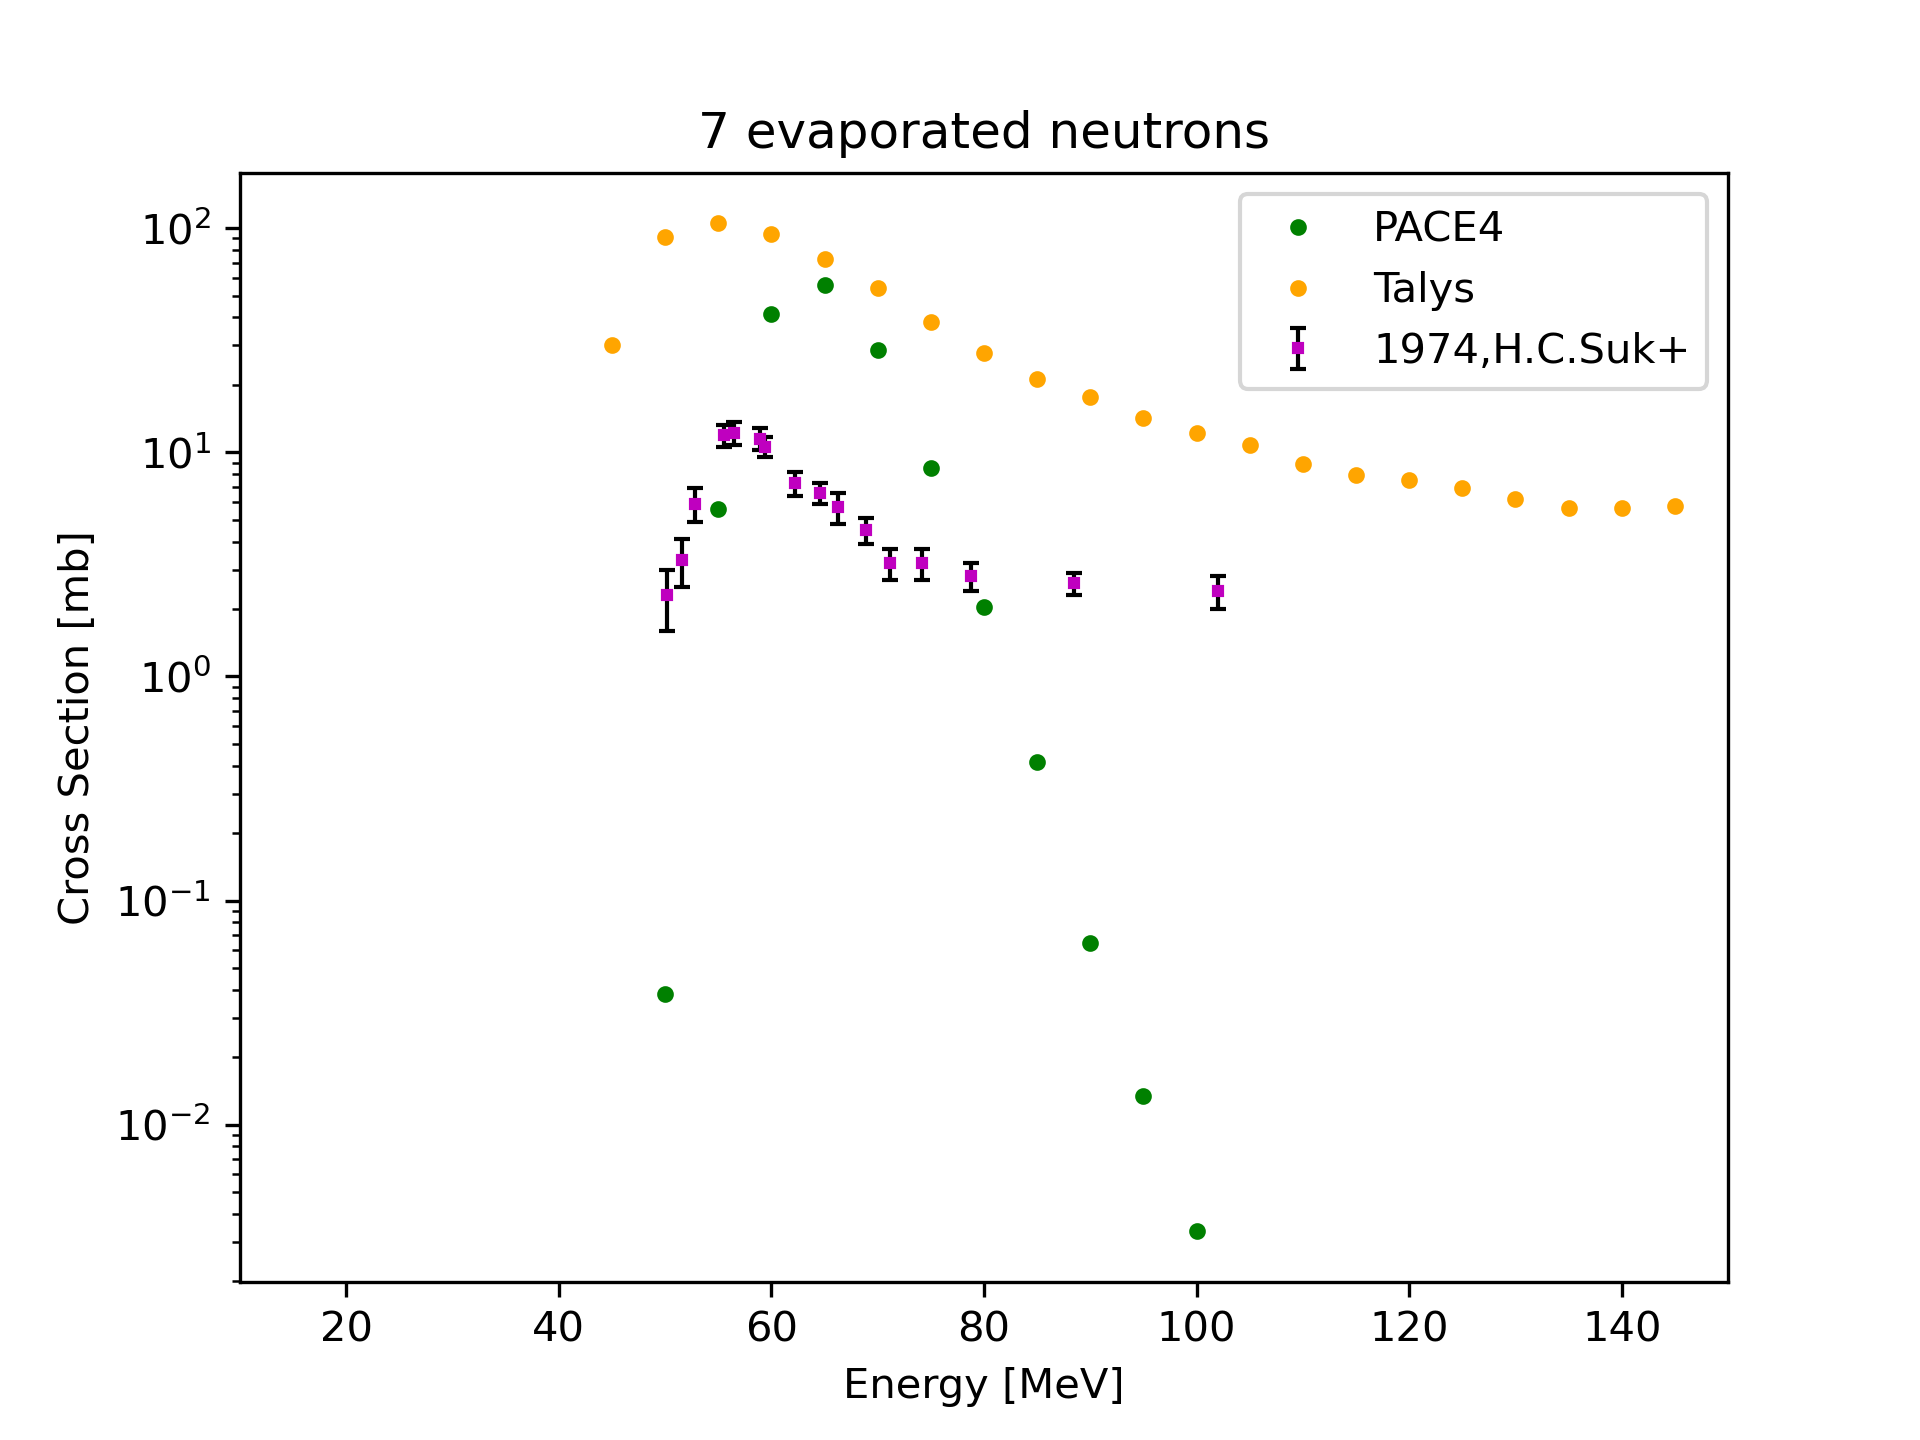
\includegraphics[width=1.2\textwidth]{232Th/091226}\\
				\vspace{0.05\textheight}		
				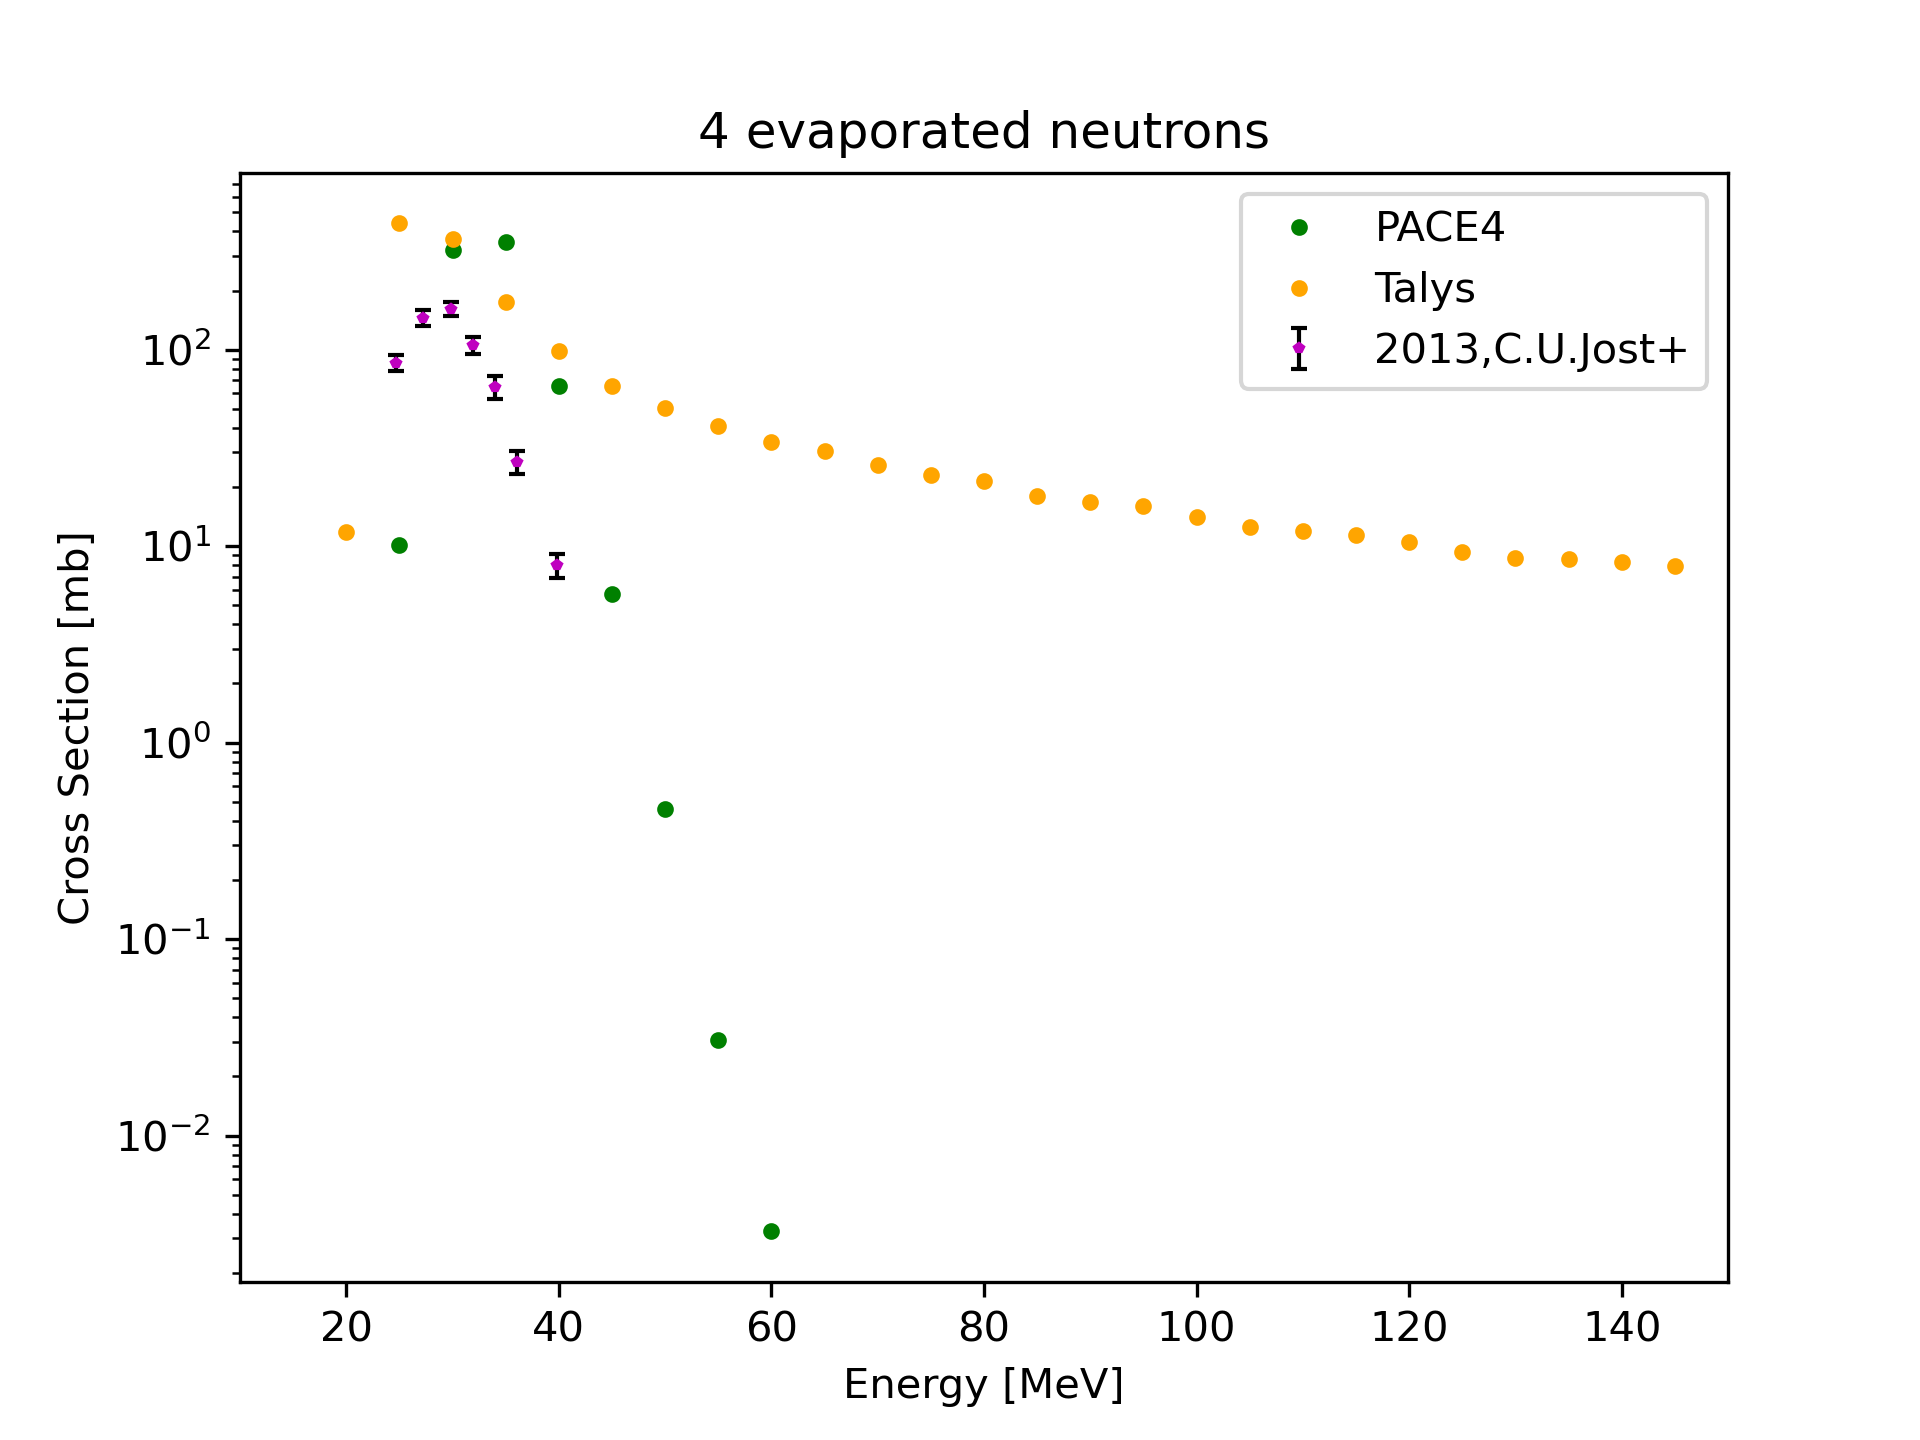
\includegraphics[width=1.2\textwidth]{232Th/091229}
			\end{overlayarea}
		\end{column}
		\begin{column}{0.3\textwidth}
			\begin{overlayarea}{\textwidth}{\textheight}
				\centering	    
			   	\vspace{-0.1\textheight}
			   	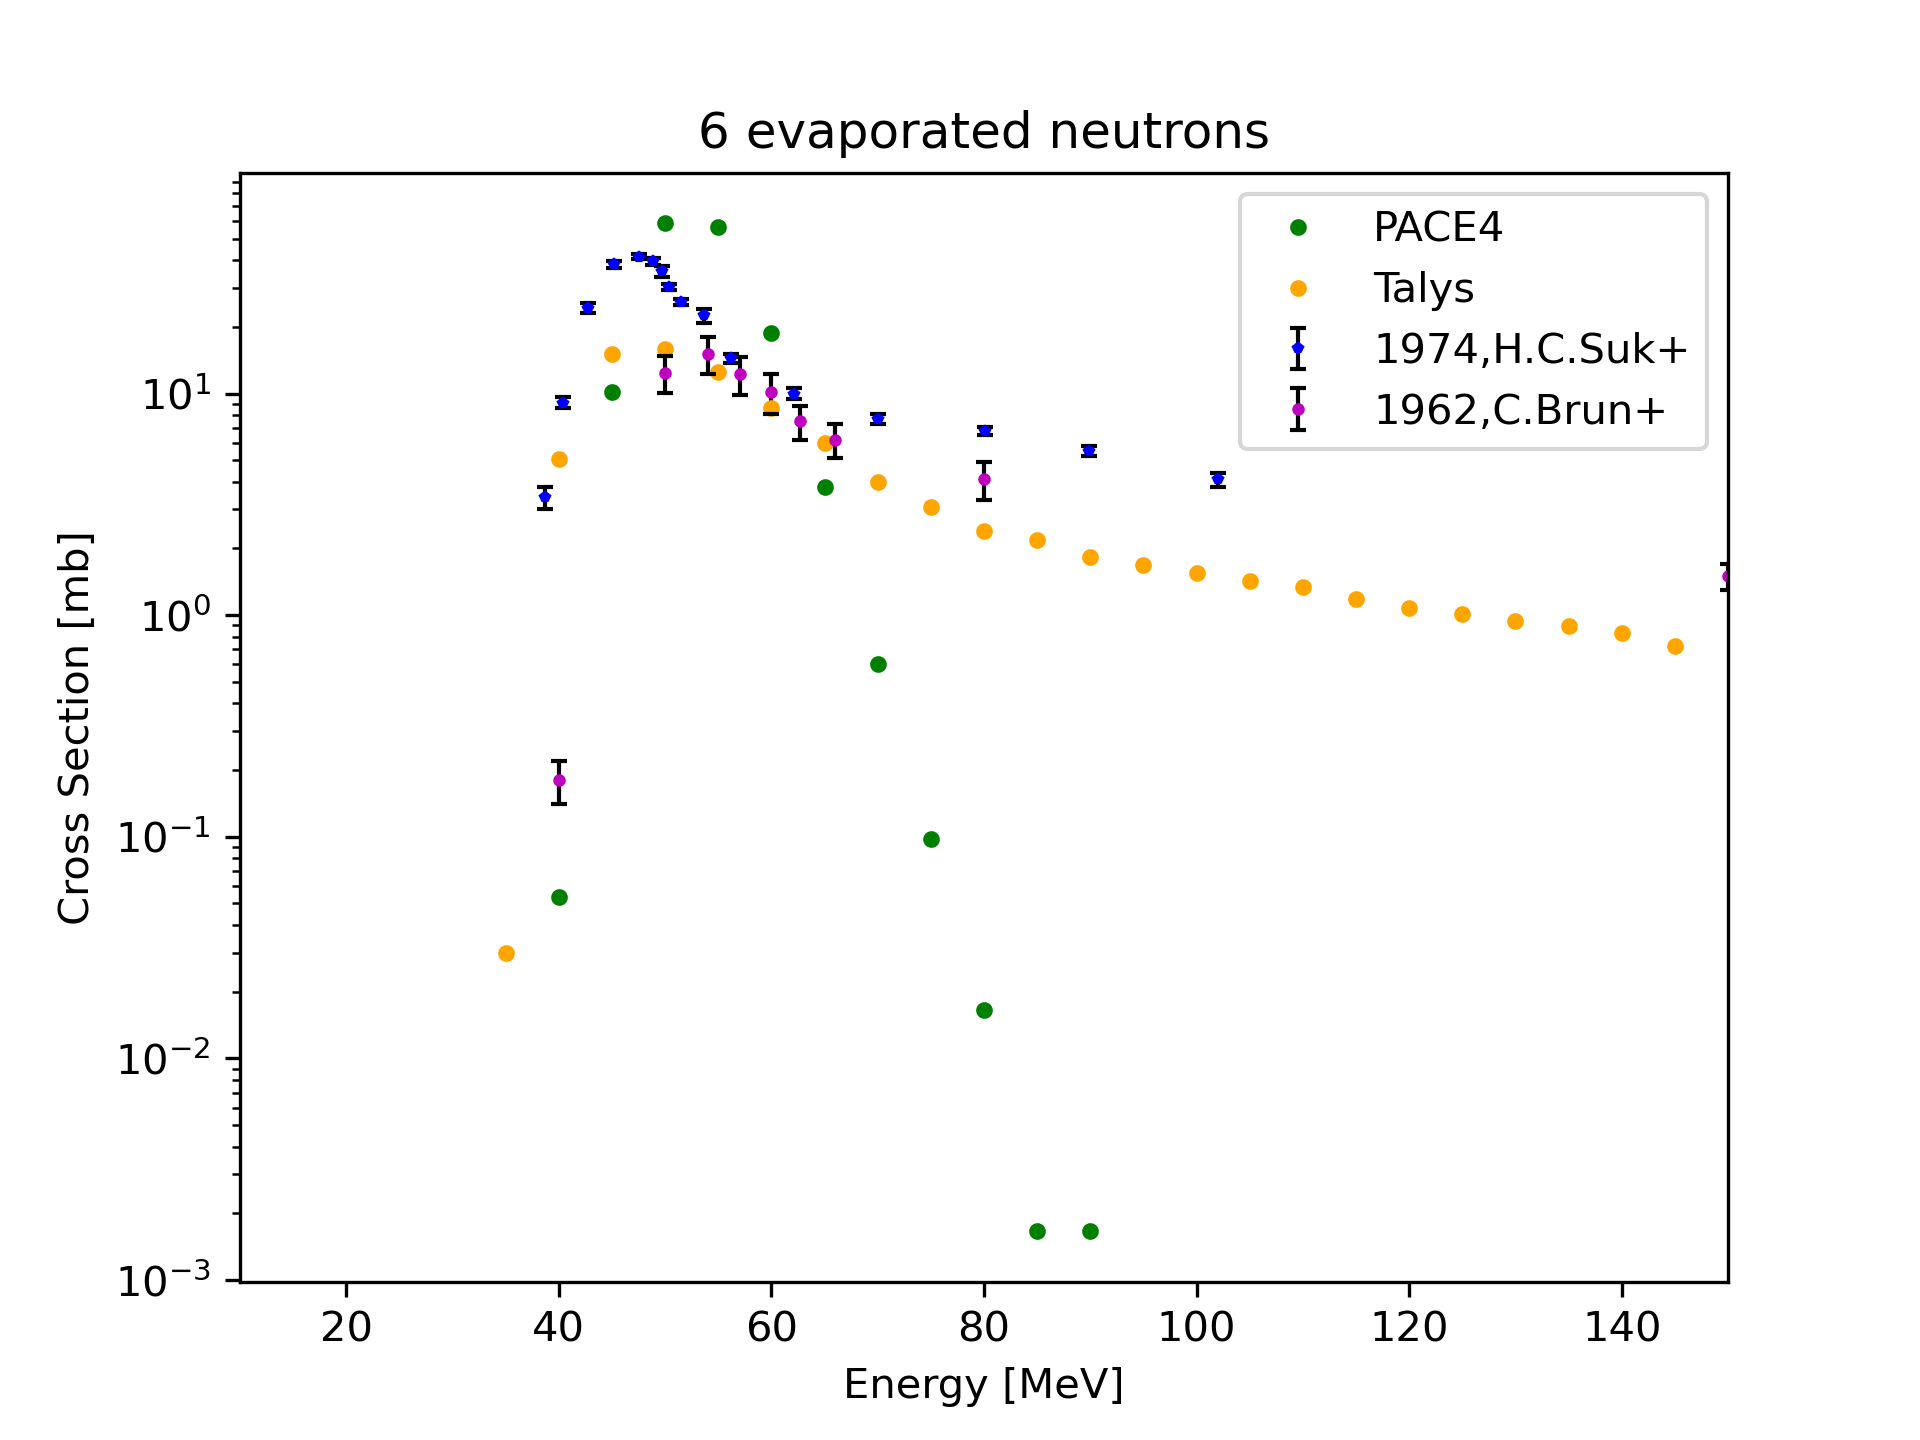
\includegraphics[width=1.2\textwidth]{232Th/091227}\\
				\vspace{0.05\textheight}				
				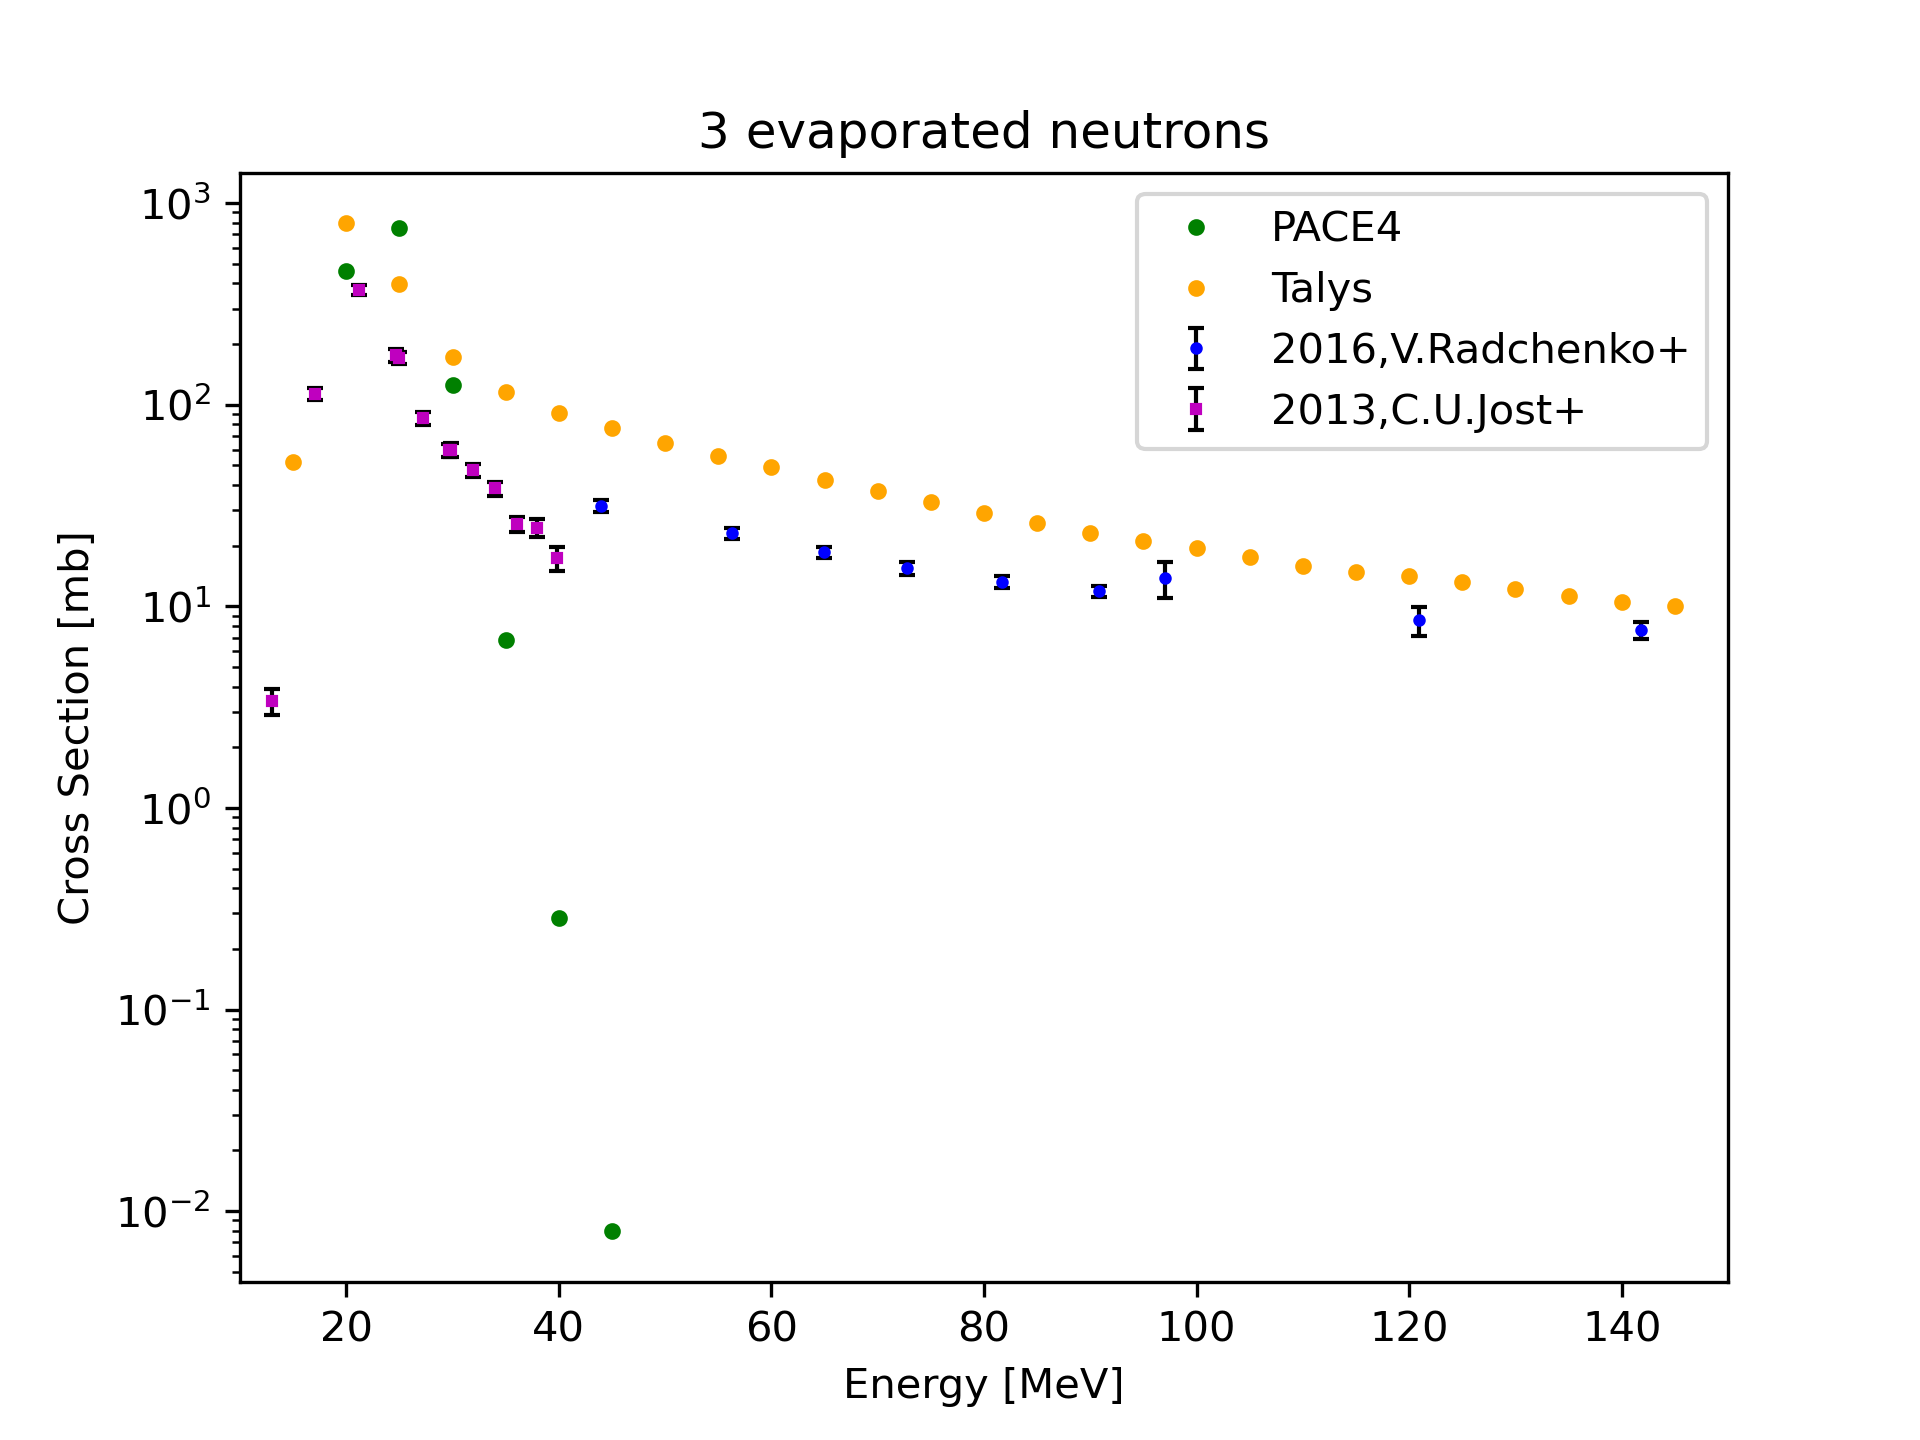
\includegraphics[width=1.2\textwidth]{232Th/091230}
			\end{overlayarea}
		\end{column}
		\begin{column}{0.3\textwidth}
			\begin{overlayarea}{\textwidth}{\textheight}
				\centering	    
			   	\vspace{-0.1\textheight}
			   	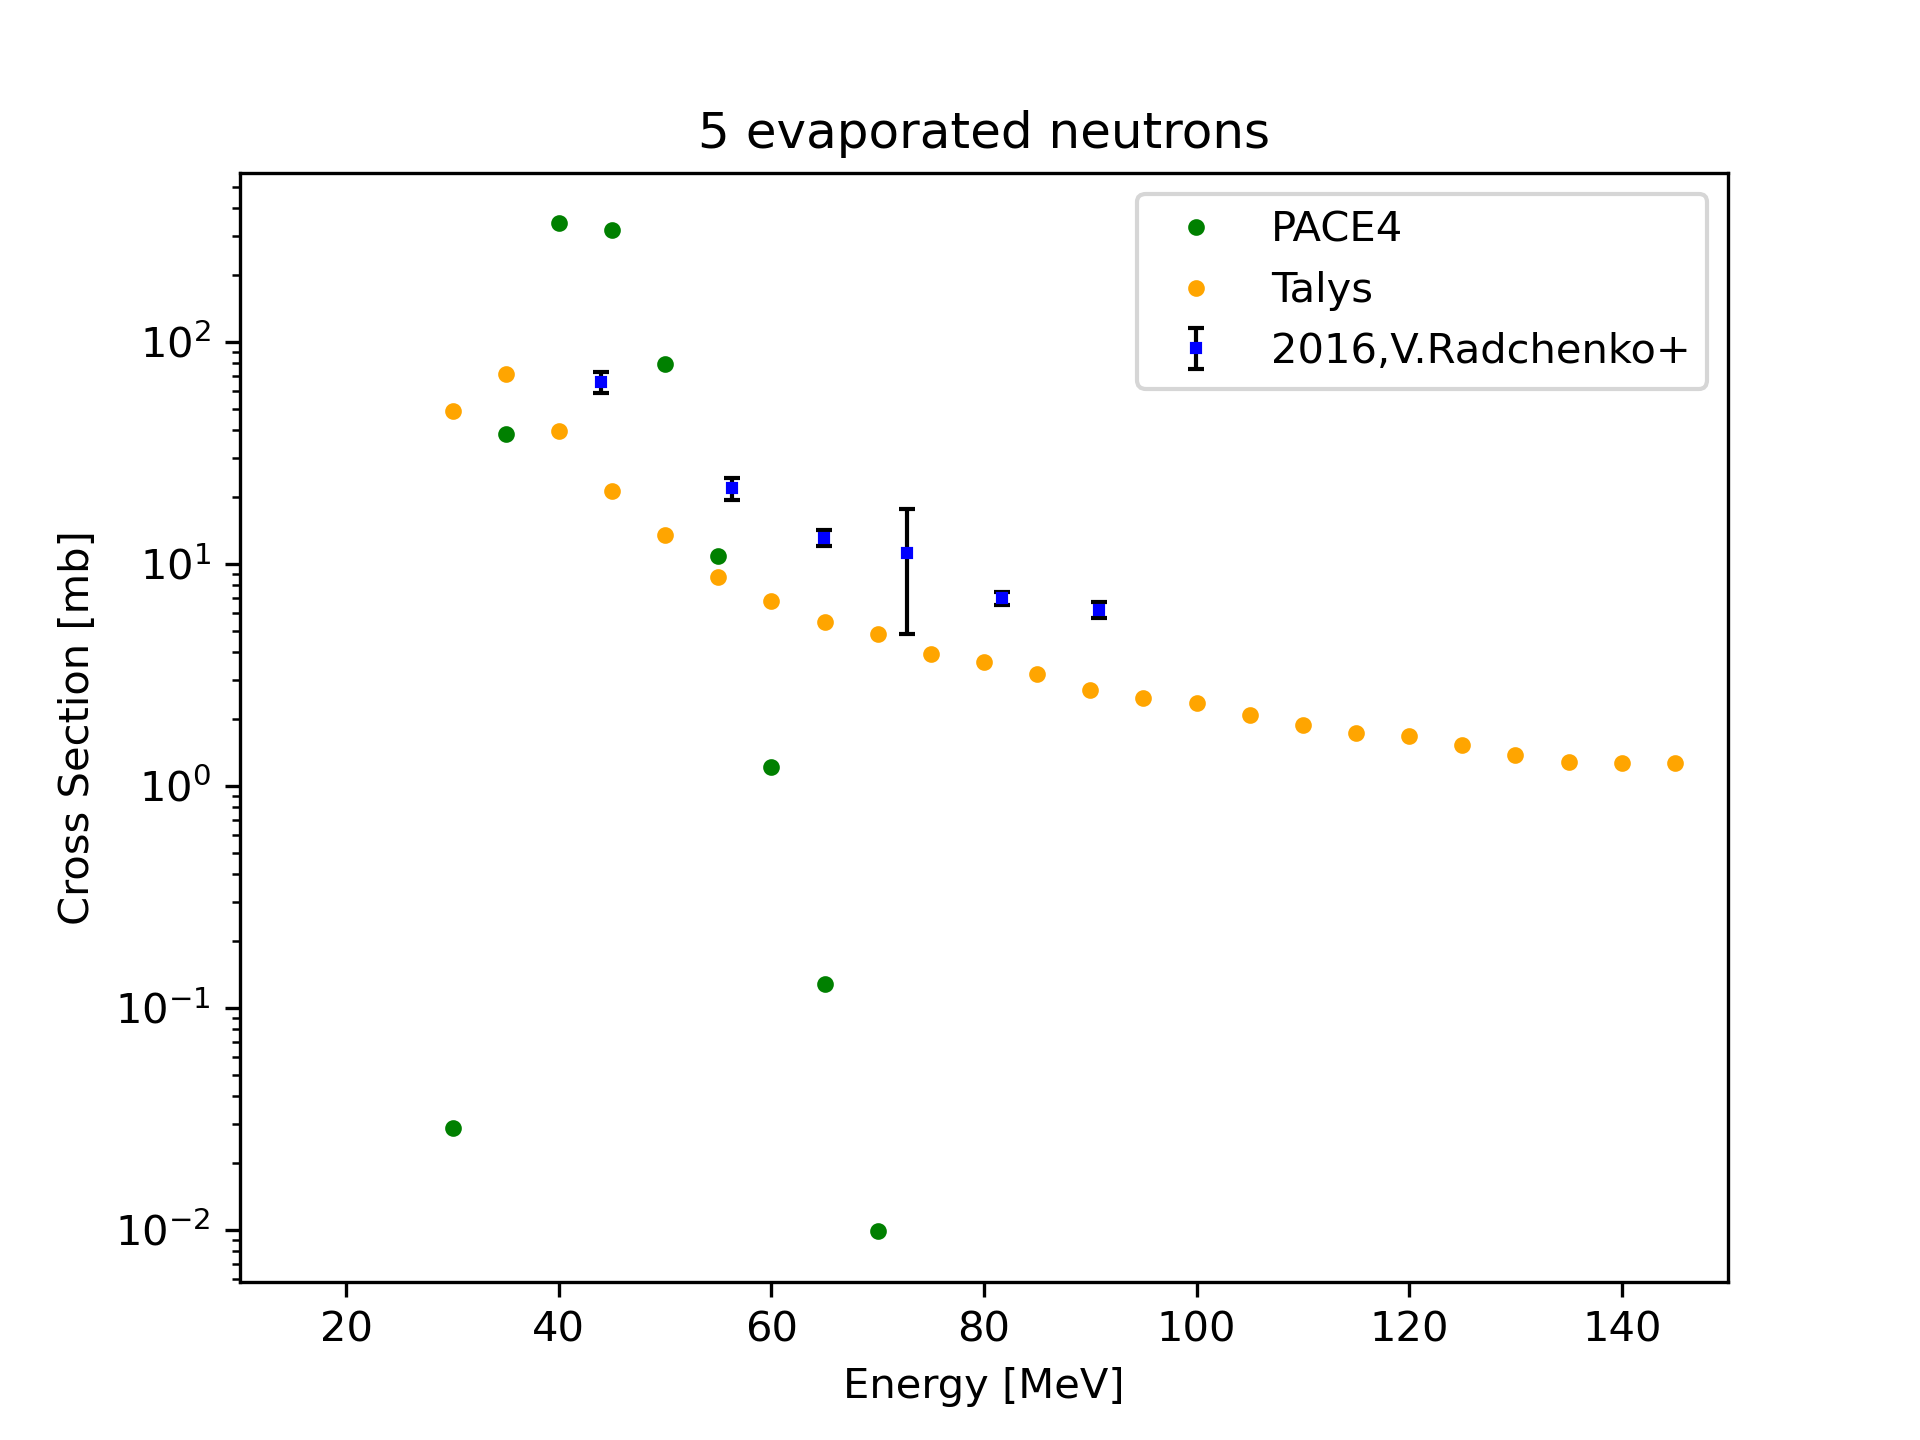
\includegraphics[width=1.2\textwidth]{232Th/091228}\\
				\vspace{0.05\textheight}				
				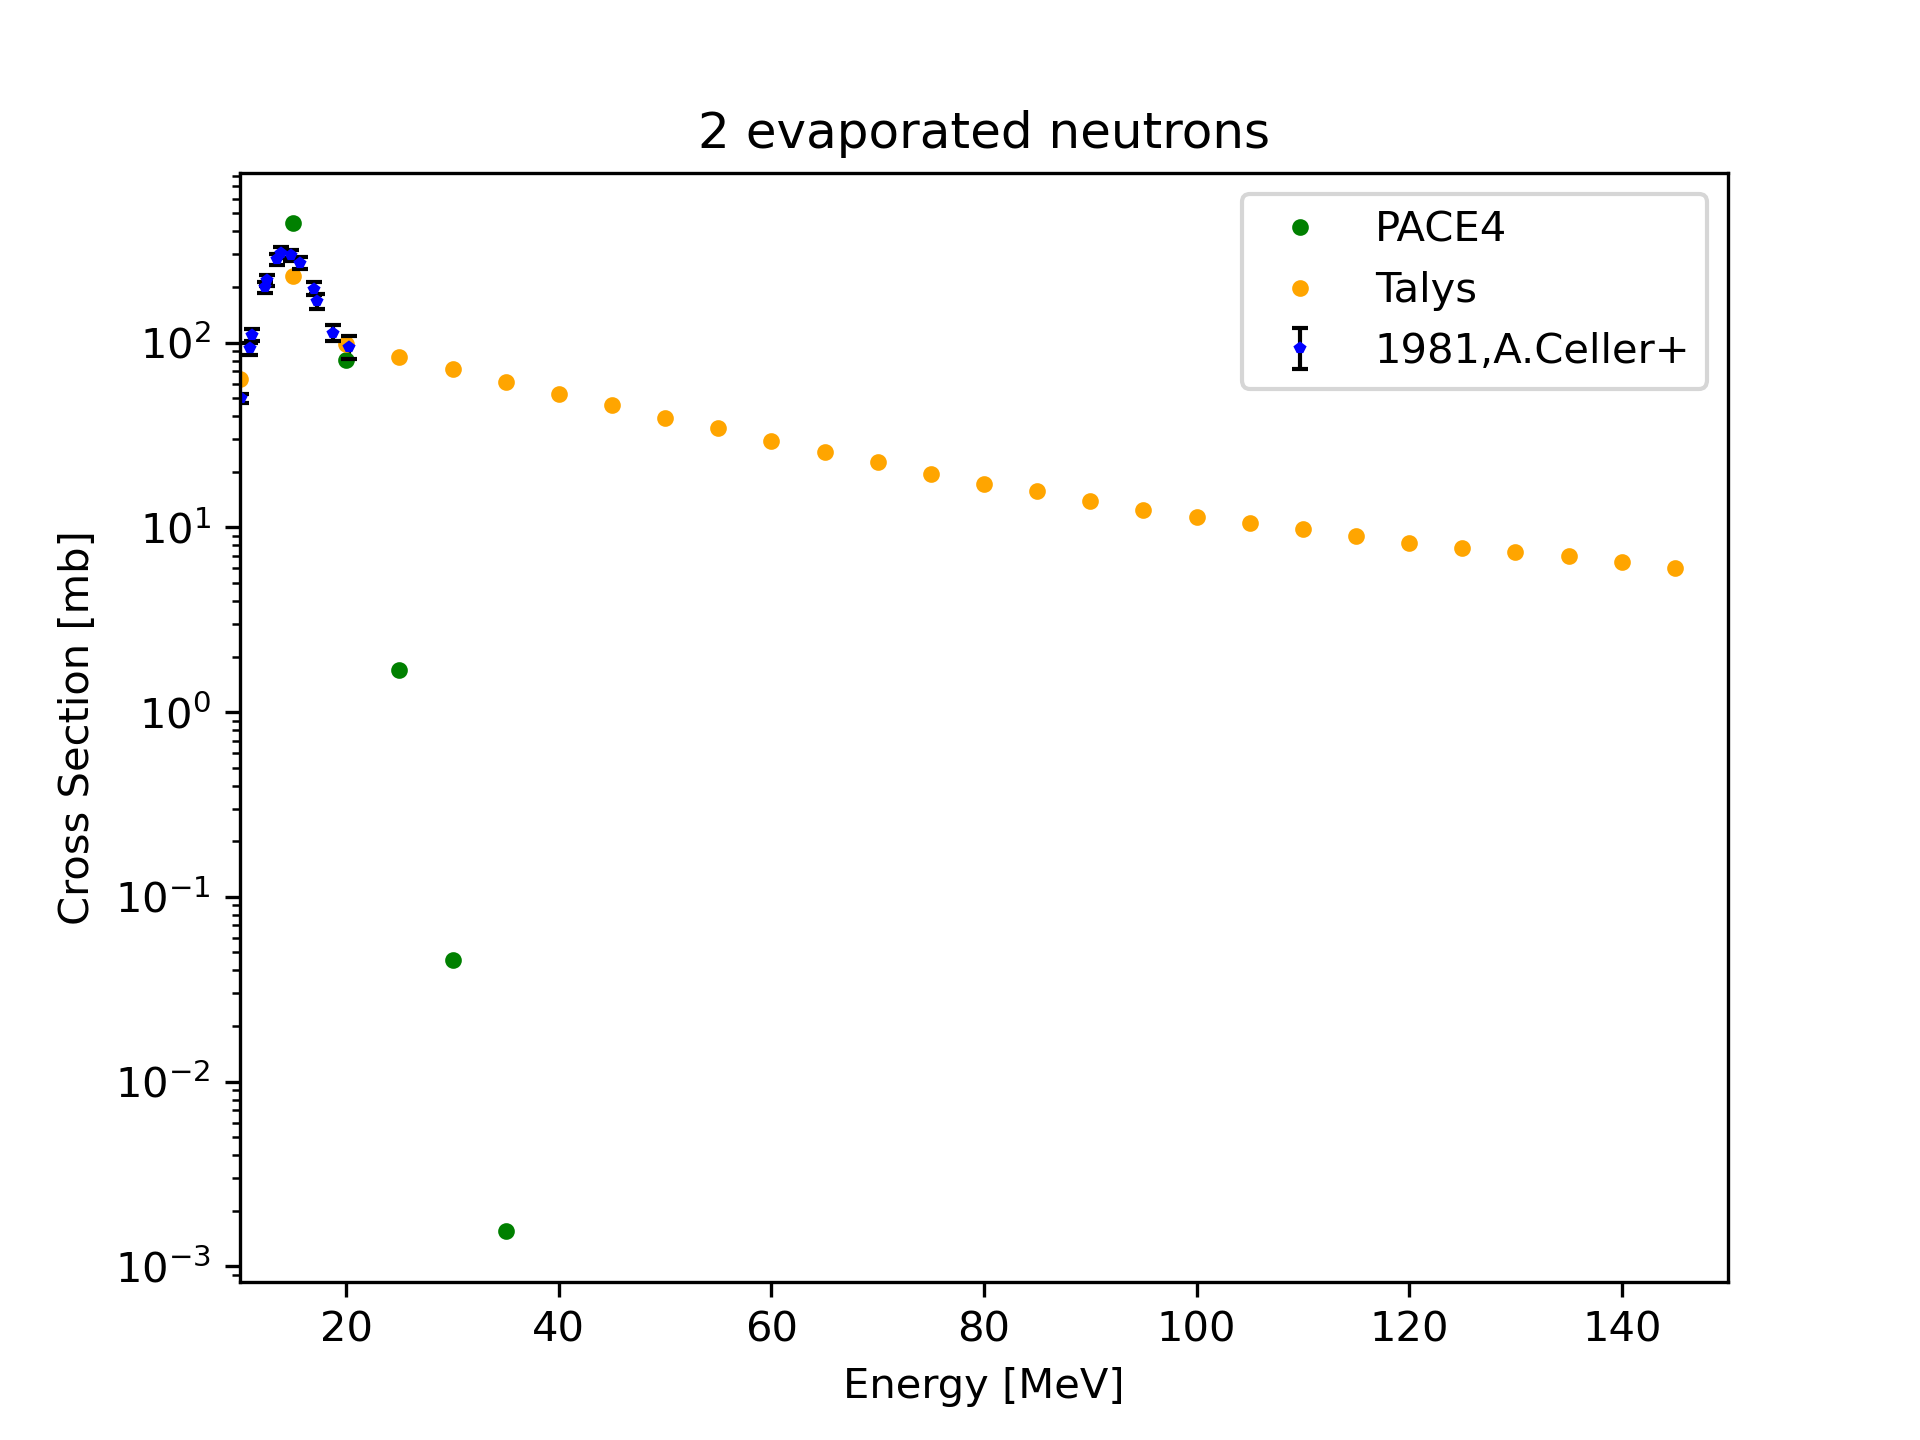
\includegraphics[width=1.2\textwidth]{232Th/091231}
			\end{overlayarea}	
		\end{column}
	\end{columns}
\end{frame}


\begin{frame}{233U+p}
	\begin{columns}
		\begin{column}{0.3\textwidth}
			\begin{overlayarea}{\textwidth}{\textheight}
				\centering	    
			   	\vspace{-0.1\textheight}
			   	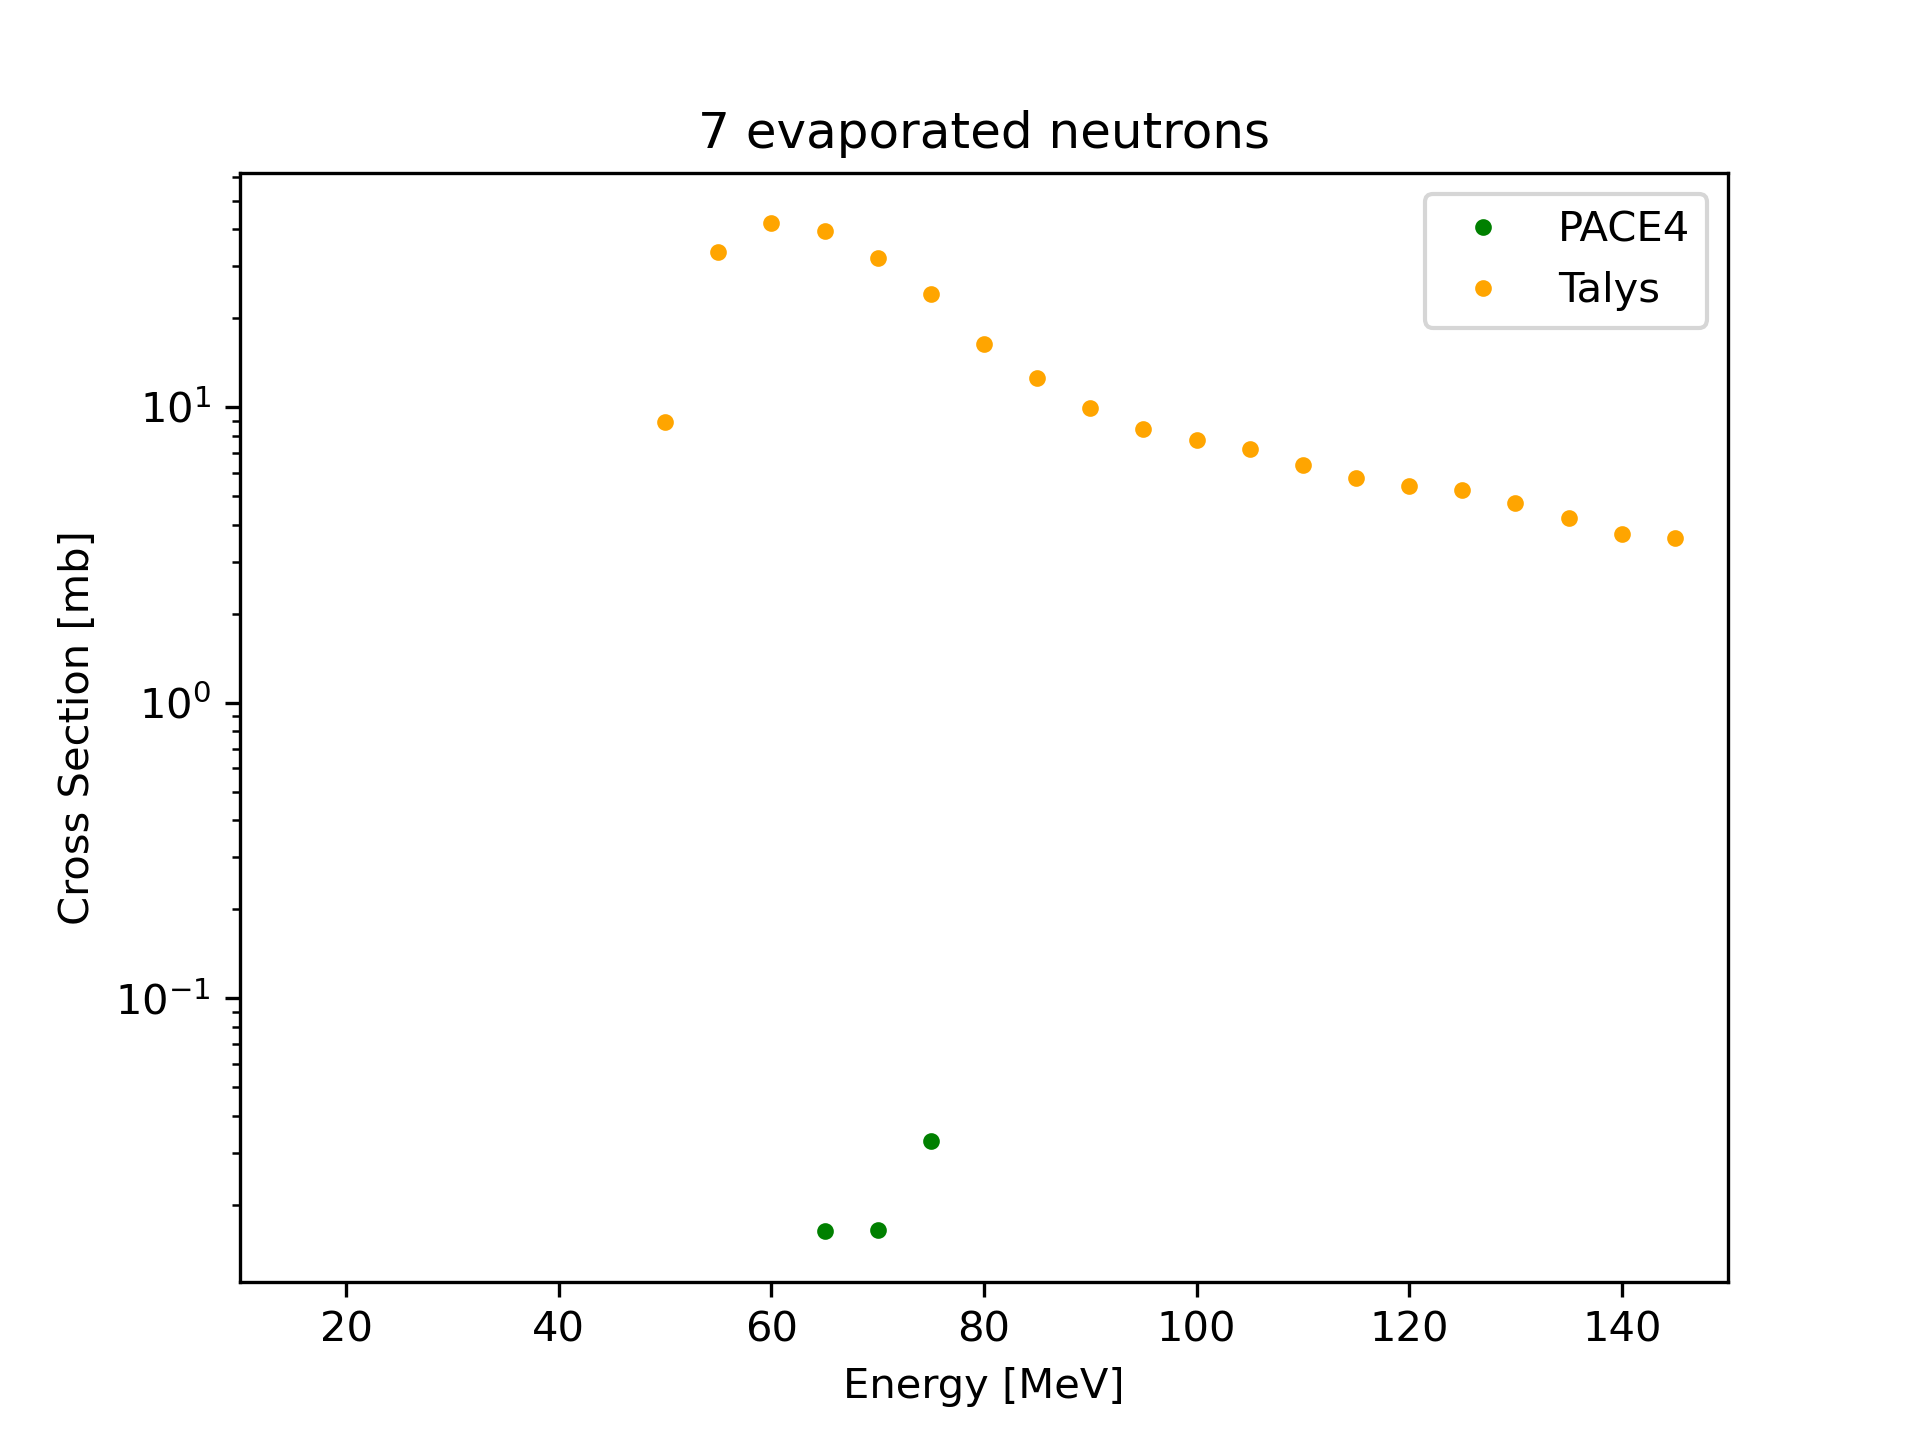
\includegraphics[width=1.2\textwidth]{233U/093227}\\
				\vspace{0.05\textheight}		
				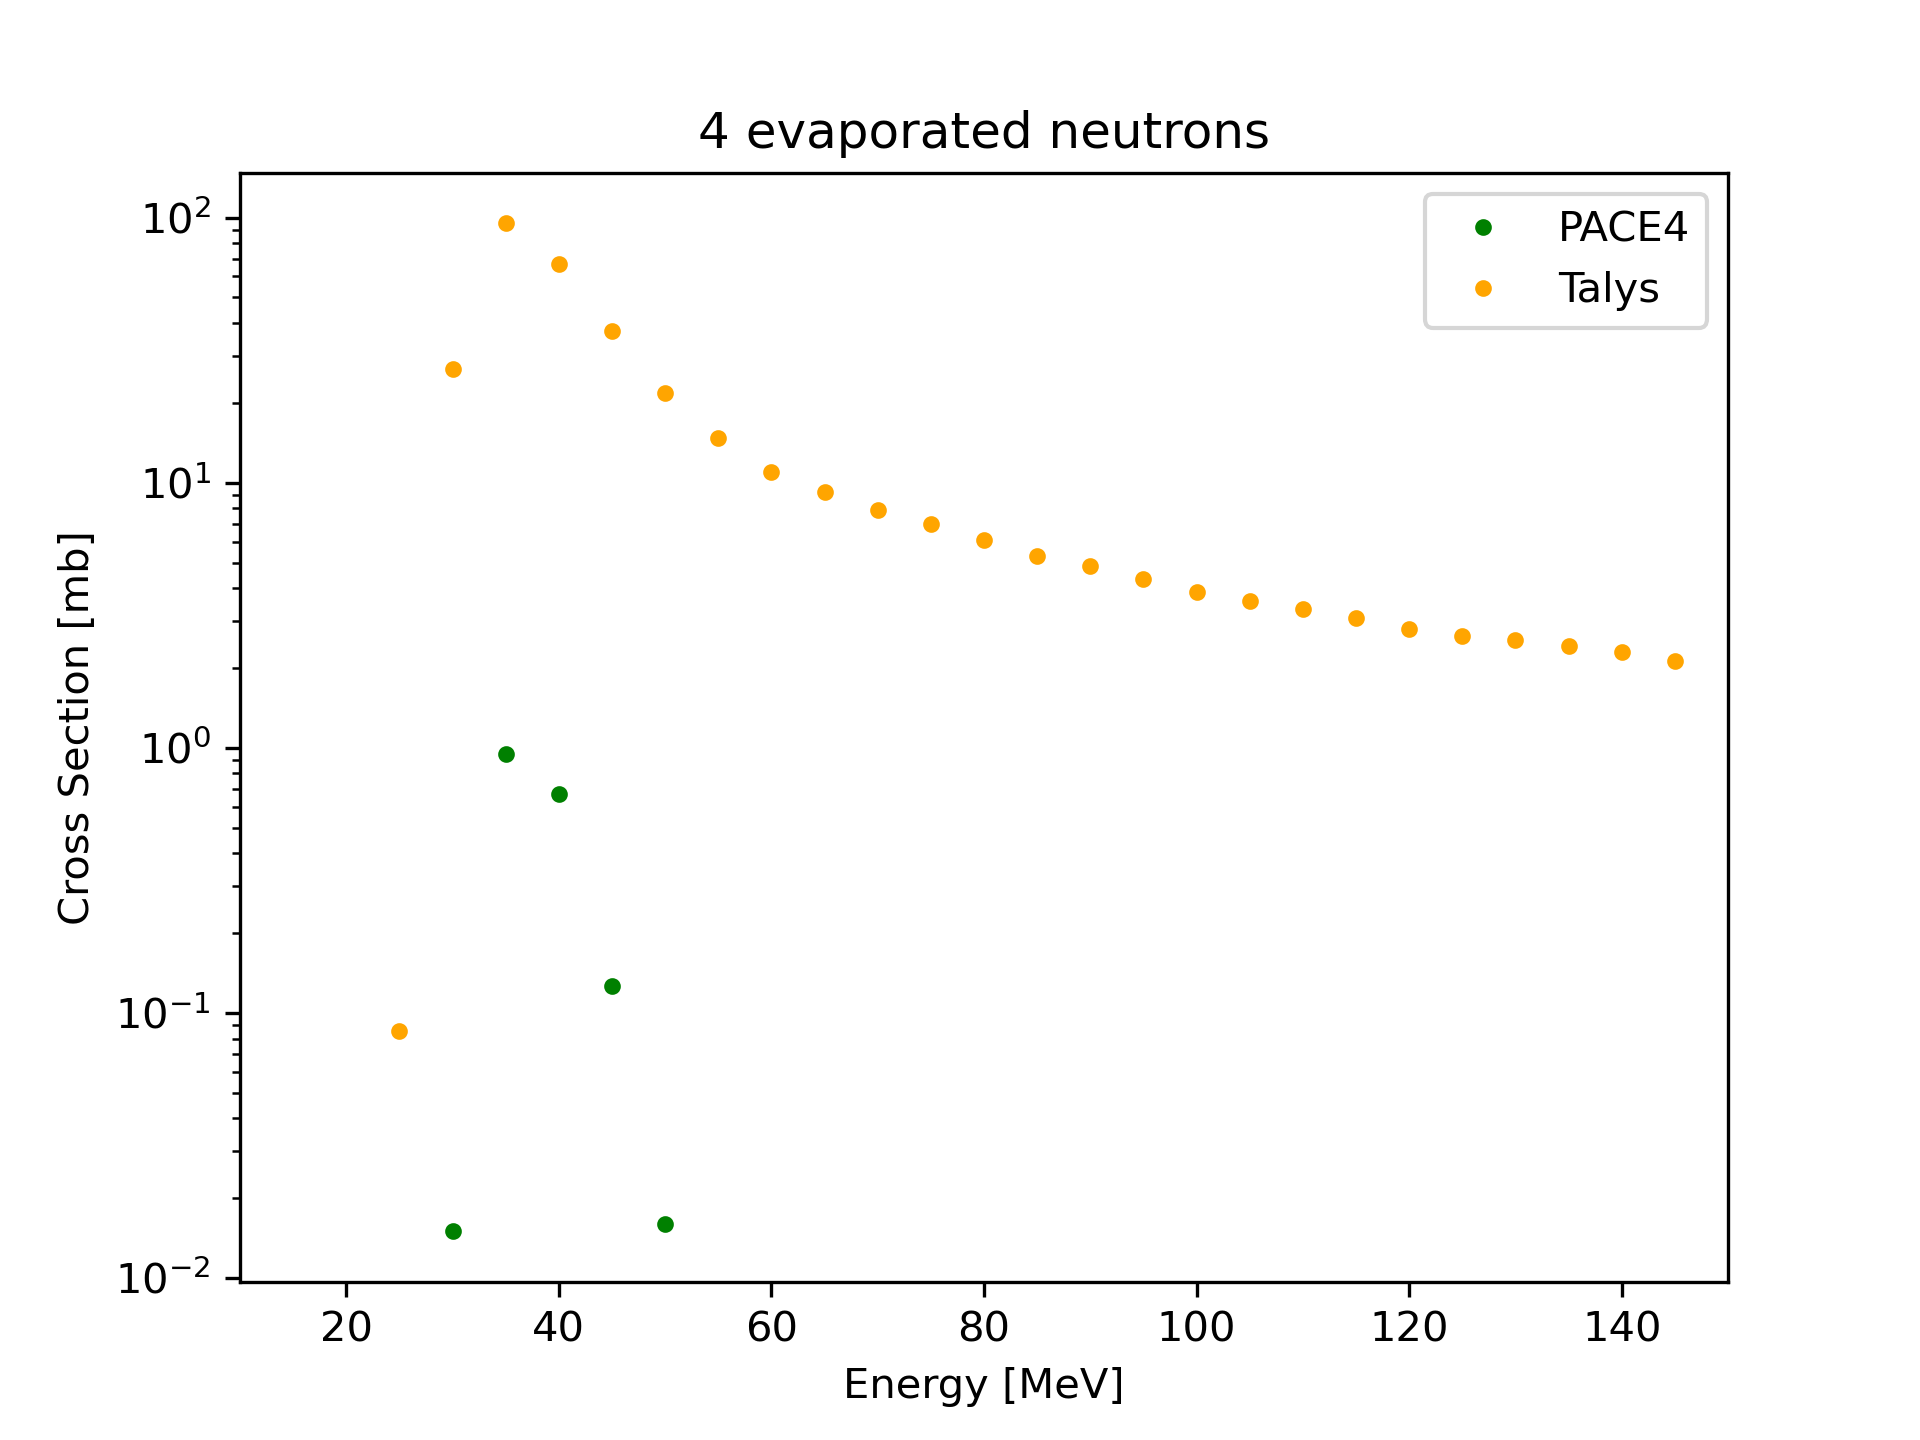
\includegraphics[width=1.2\textwidth]{233U/093230}
			\end{overlayarea}
		\end{column}
		\begin{column}{0.3\textwidth}
			\begin{overlayarea}{\textwidth}{\textheight}
				\centering	    
			   	\vspace{-0.1\textheight}
			   	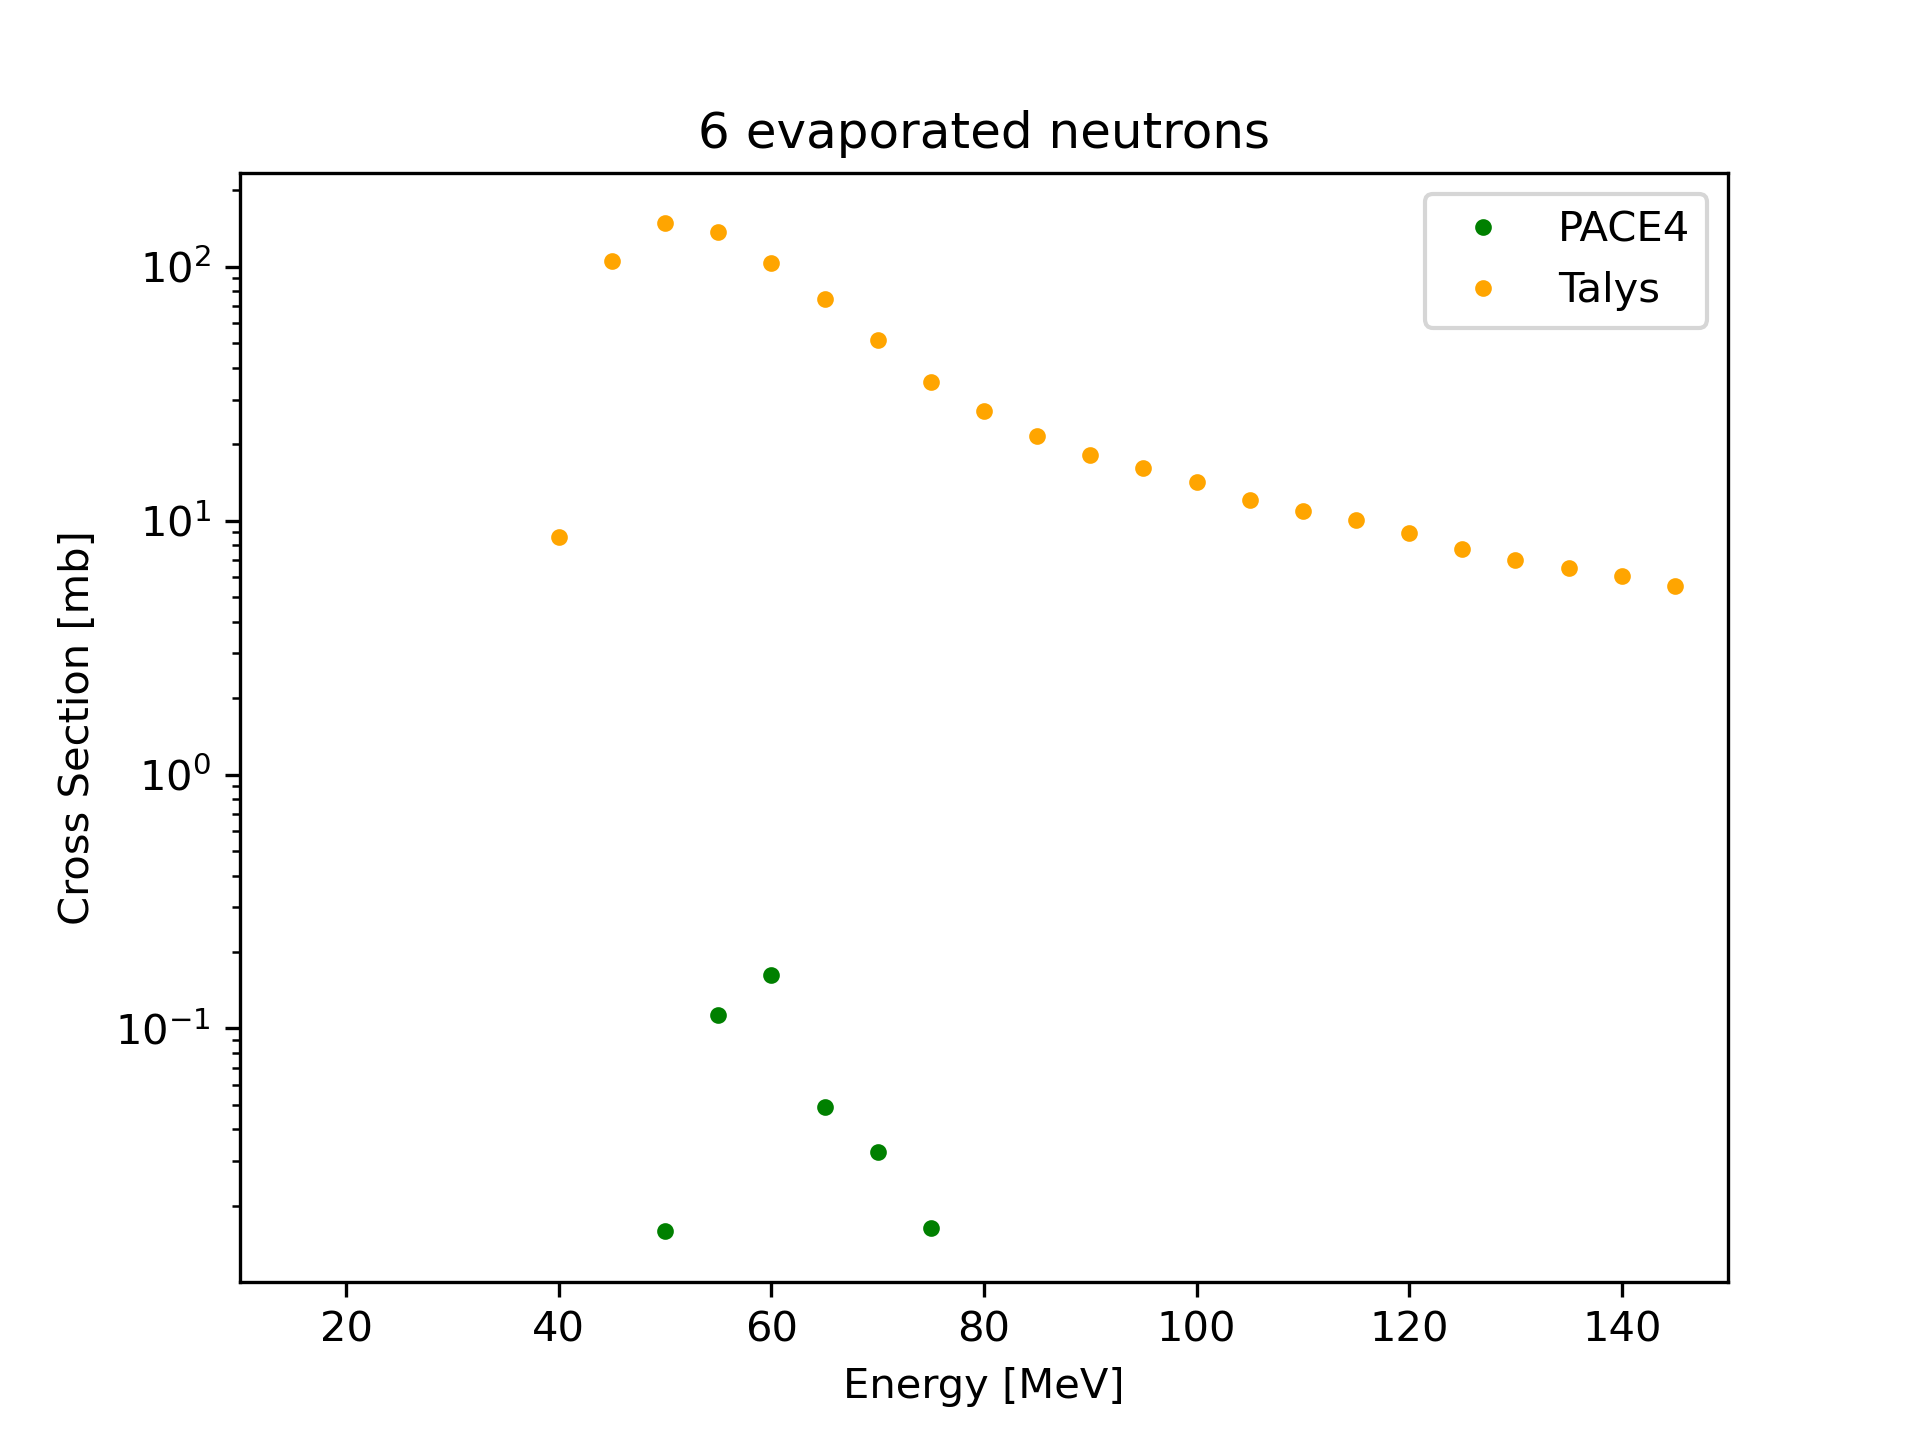
\includegraphics[width=1.2\textwidth]{233U/093228}\\
				\vspace{0.05\textheight}				
				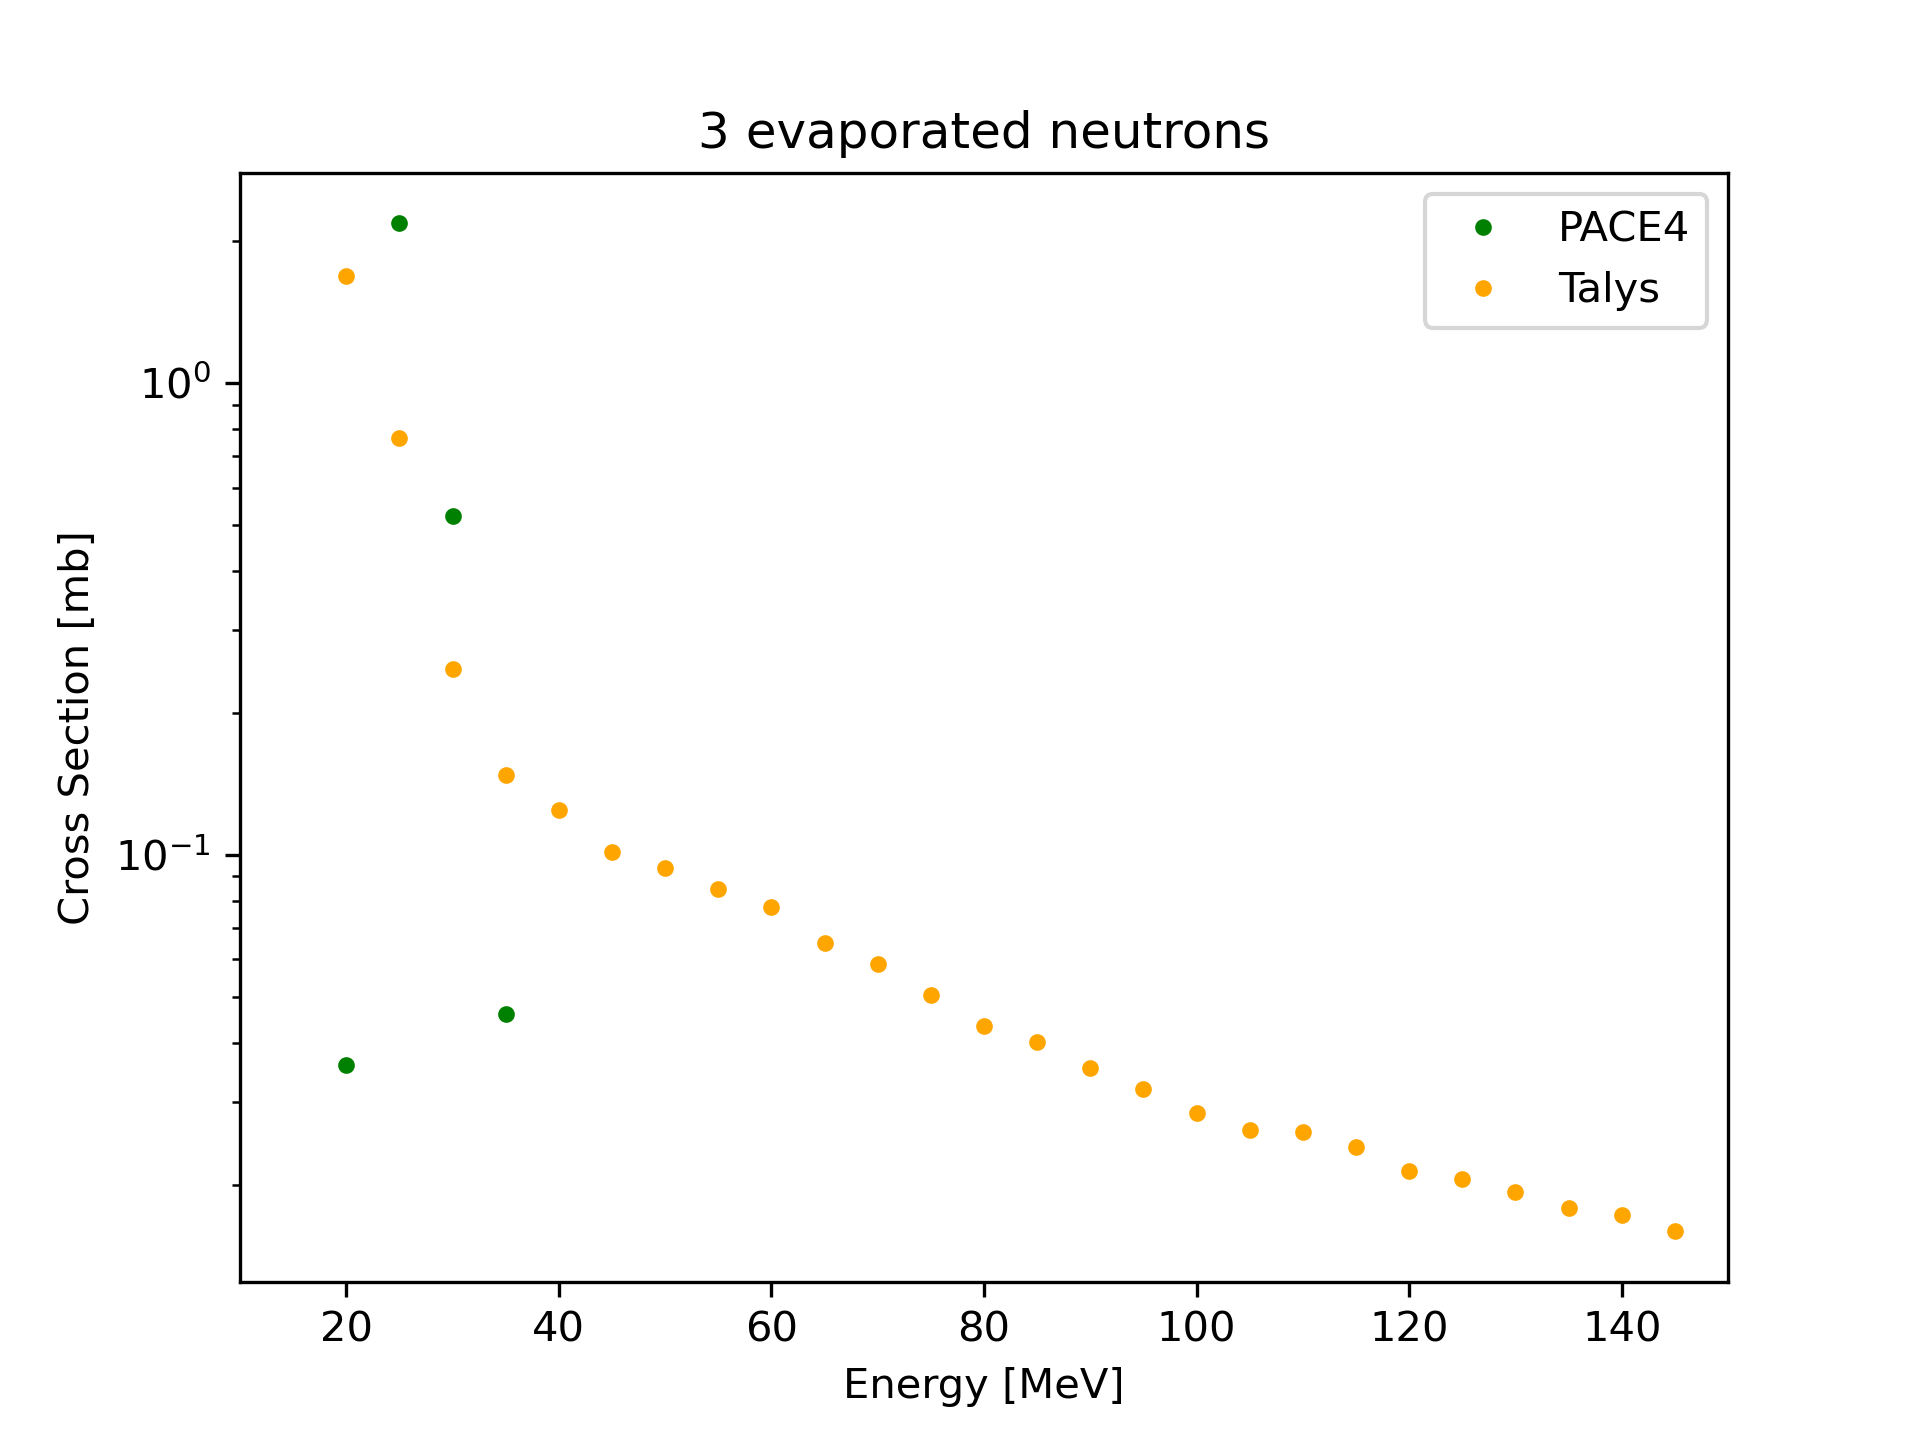
\includegraphics[width=1.2\textwidth]{233U/093231}
			\end{overlayarea}
		\end{column}
		\begin{column}{0.3\textwidth}
			\begin{overlayarea}{\textwidth}{\textheight}
				\centering	    
			   	\vspace{-0.1\textheight}
			   	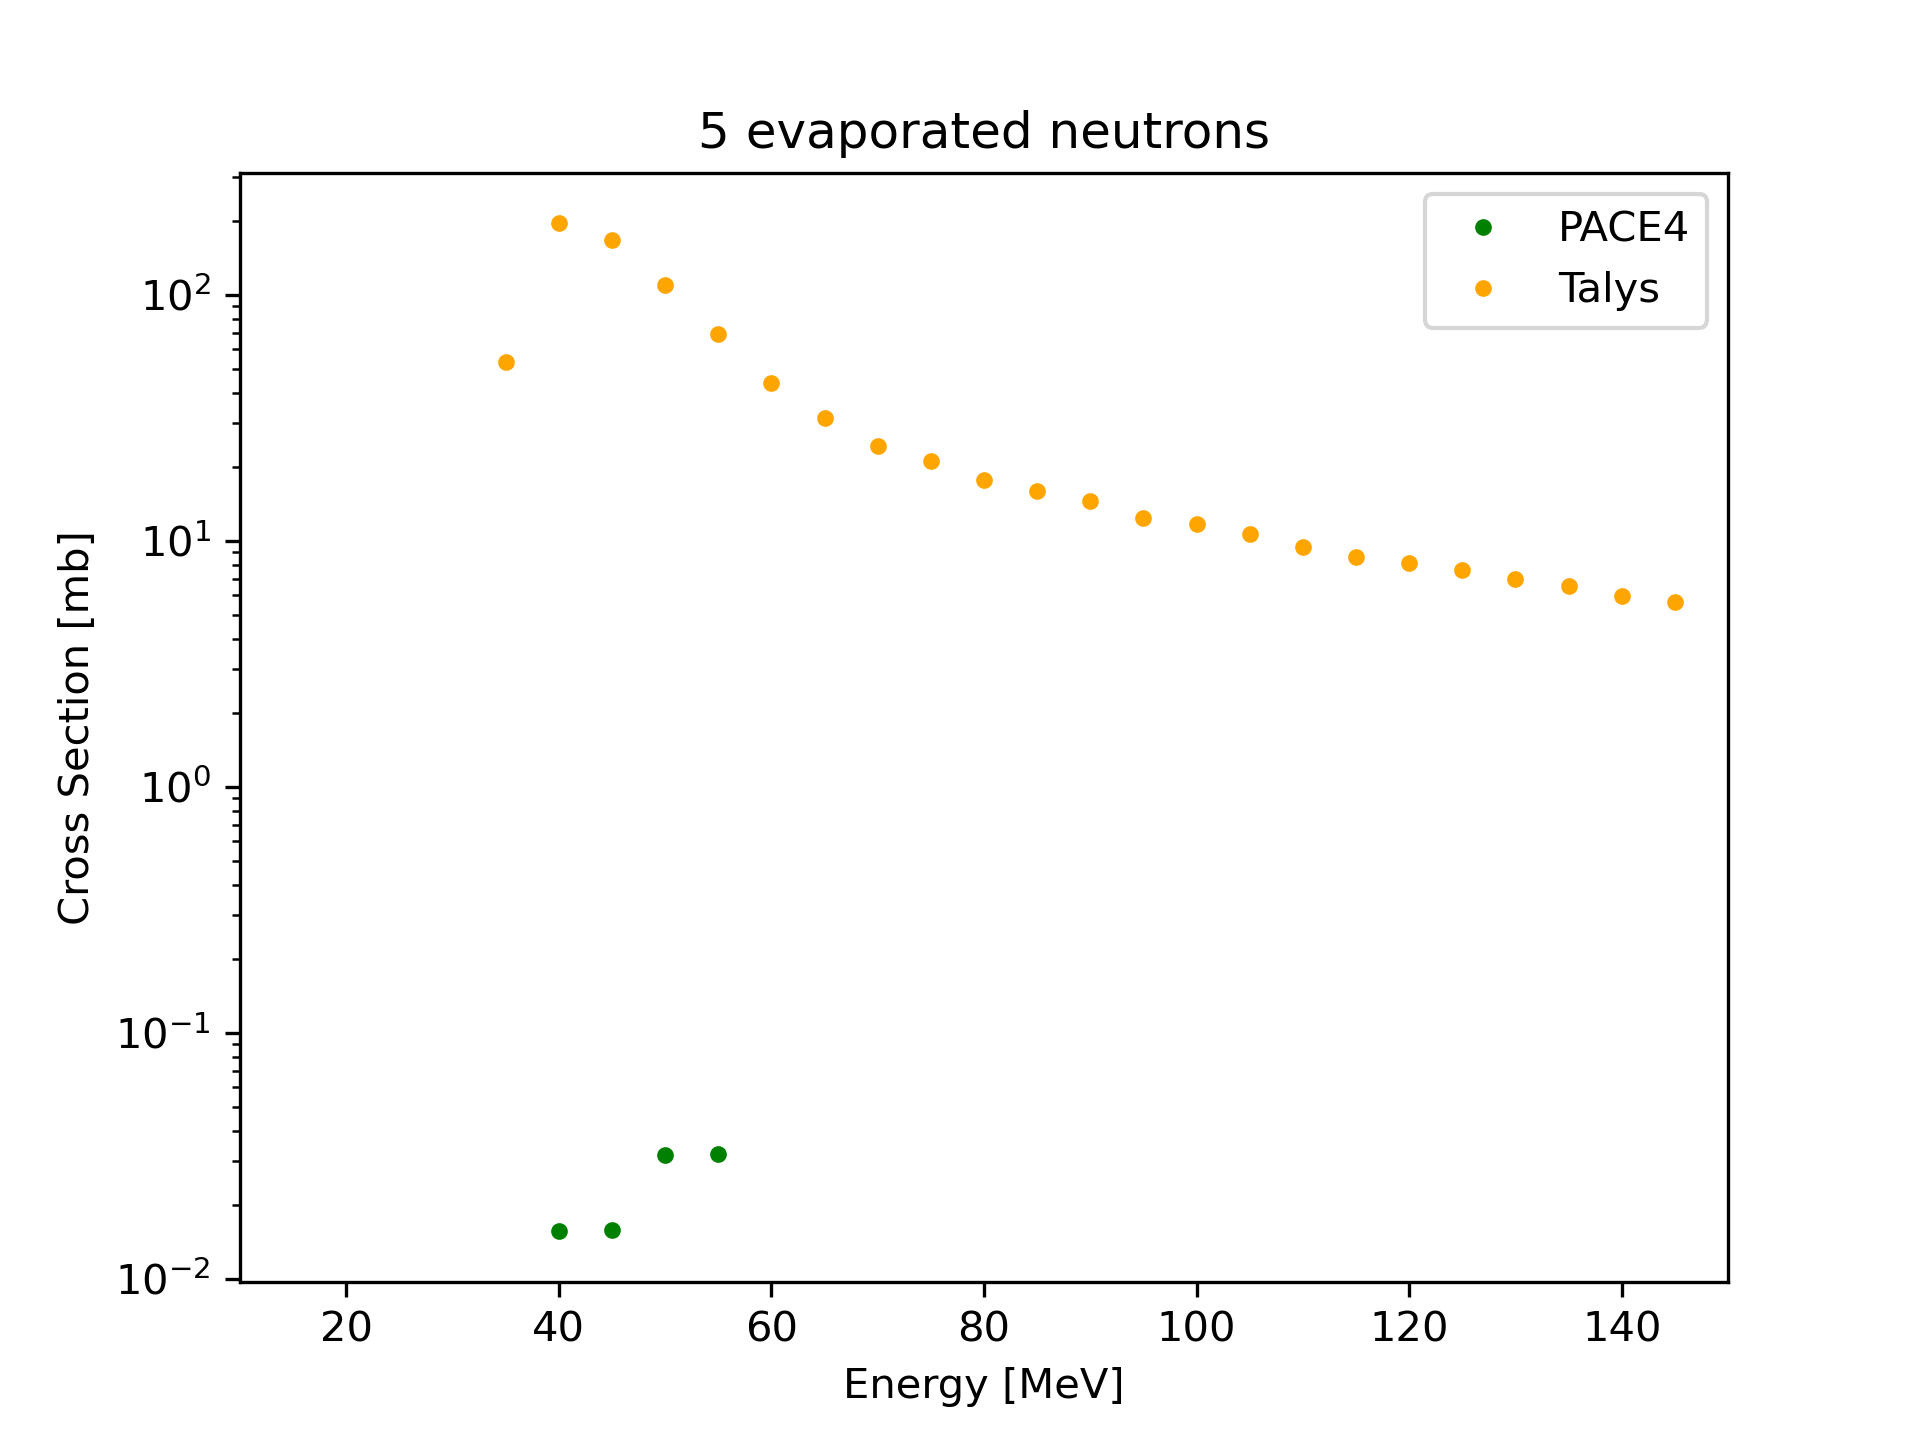
\includegraphics[width=1.2\textwidth]{233U/093229}\\
				\vspace{0.05\textheight}				
				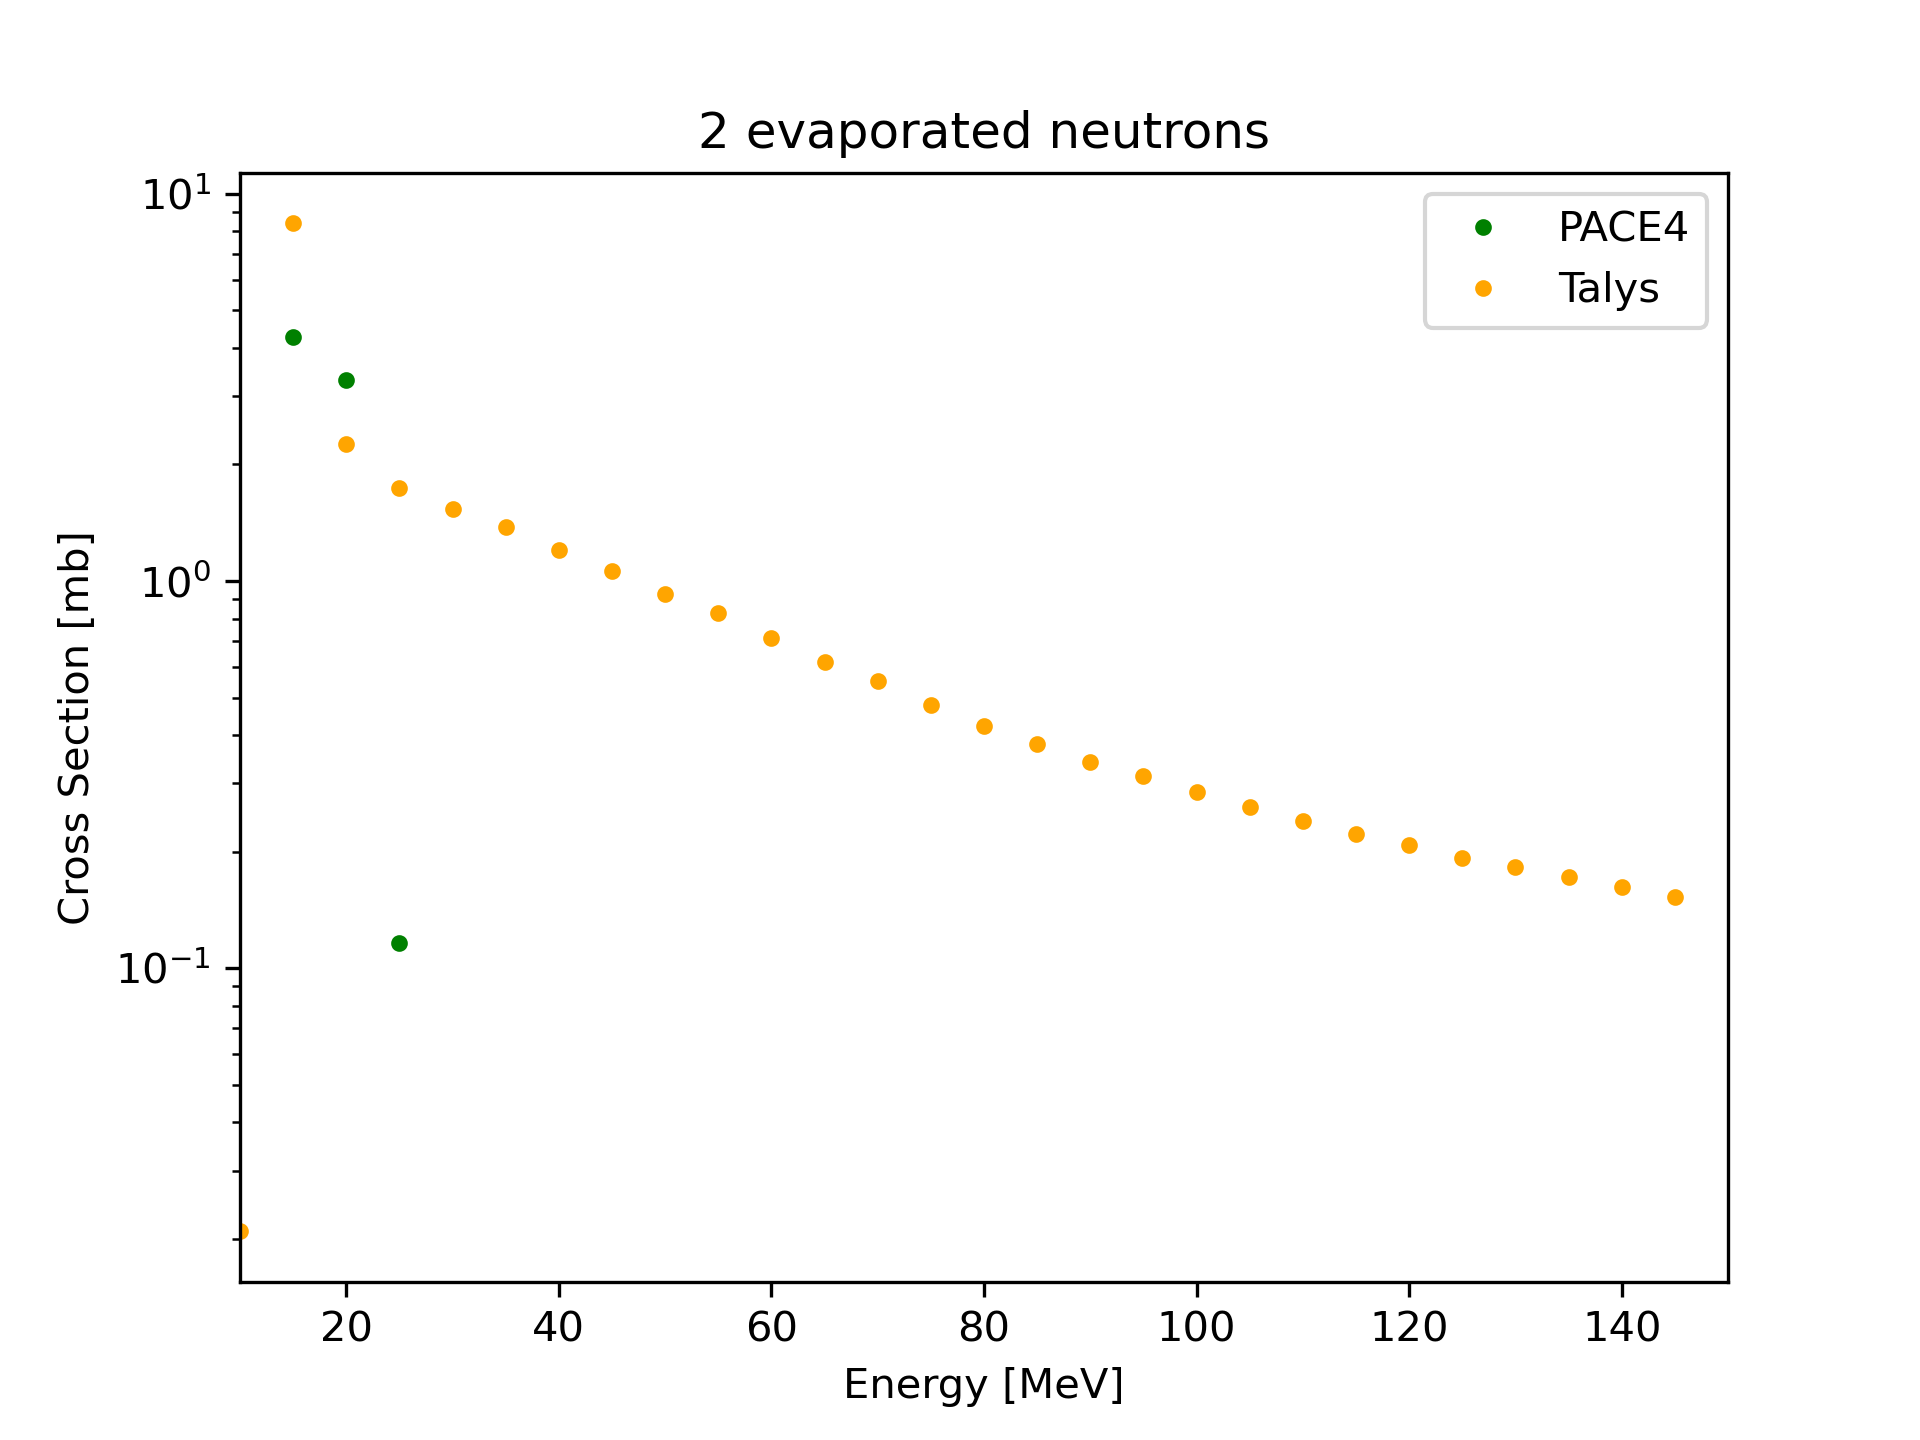
\includegraphics[width=1.2\textwidth]{233U/093232}
			\end{overlayarea}	
		\end{column}
	\end{columns}
\end{frame}

\begin{frame}{238U+p}
	\begin{columns}
		\begin{column}{0.5\textwidth}
			\begin{overlayarea}{\textwidth}{\textheight}
				\centering	    
			   	\vspace{-0.1\textheight}
			   	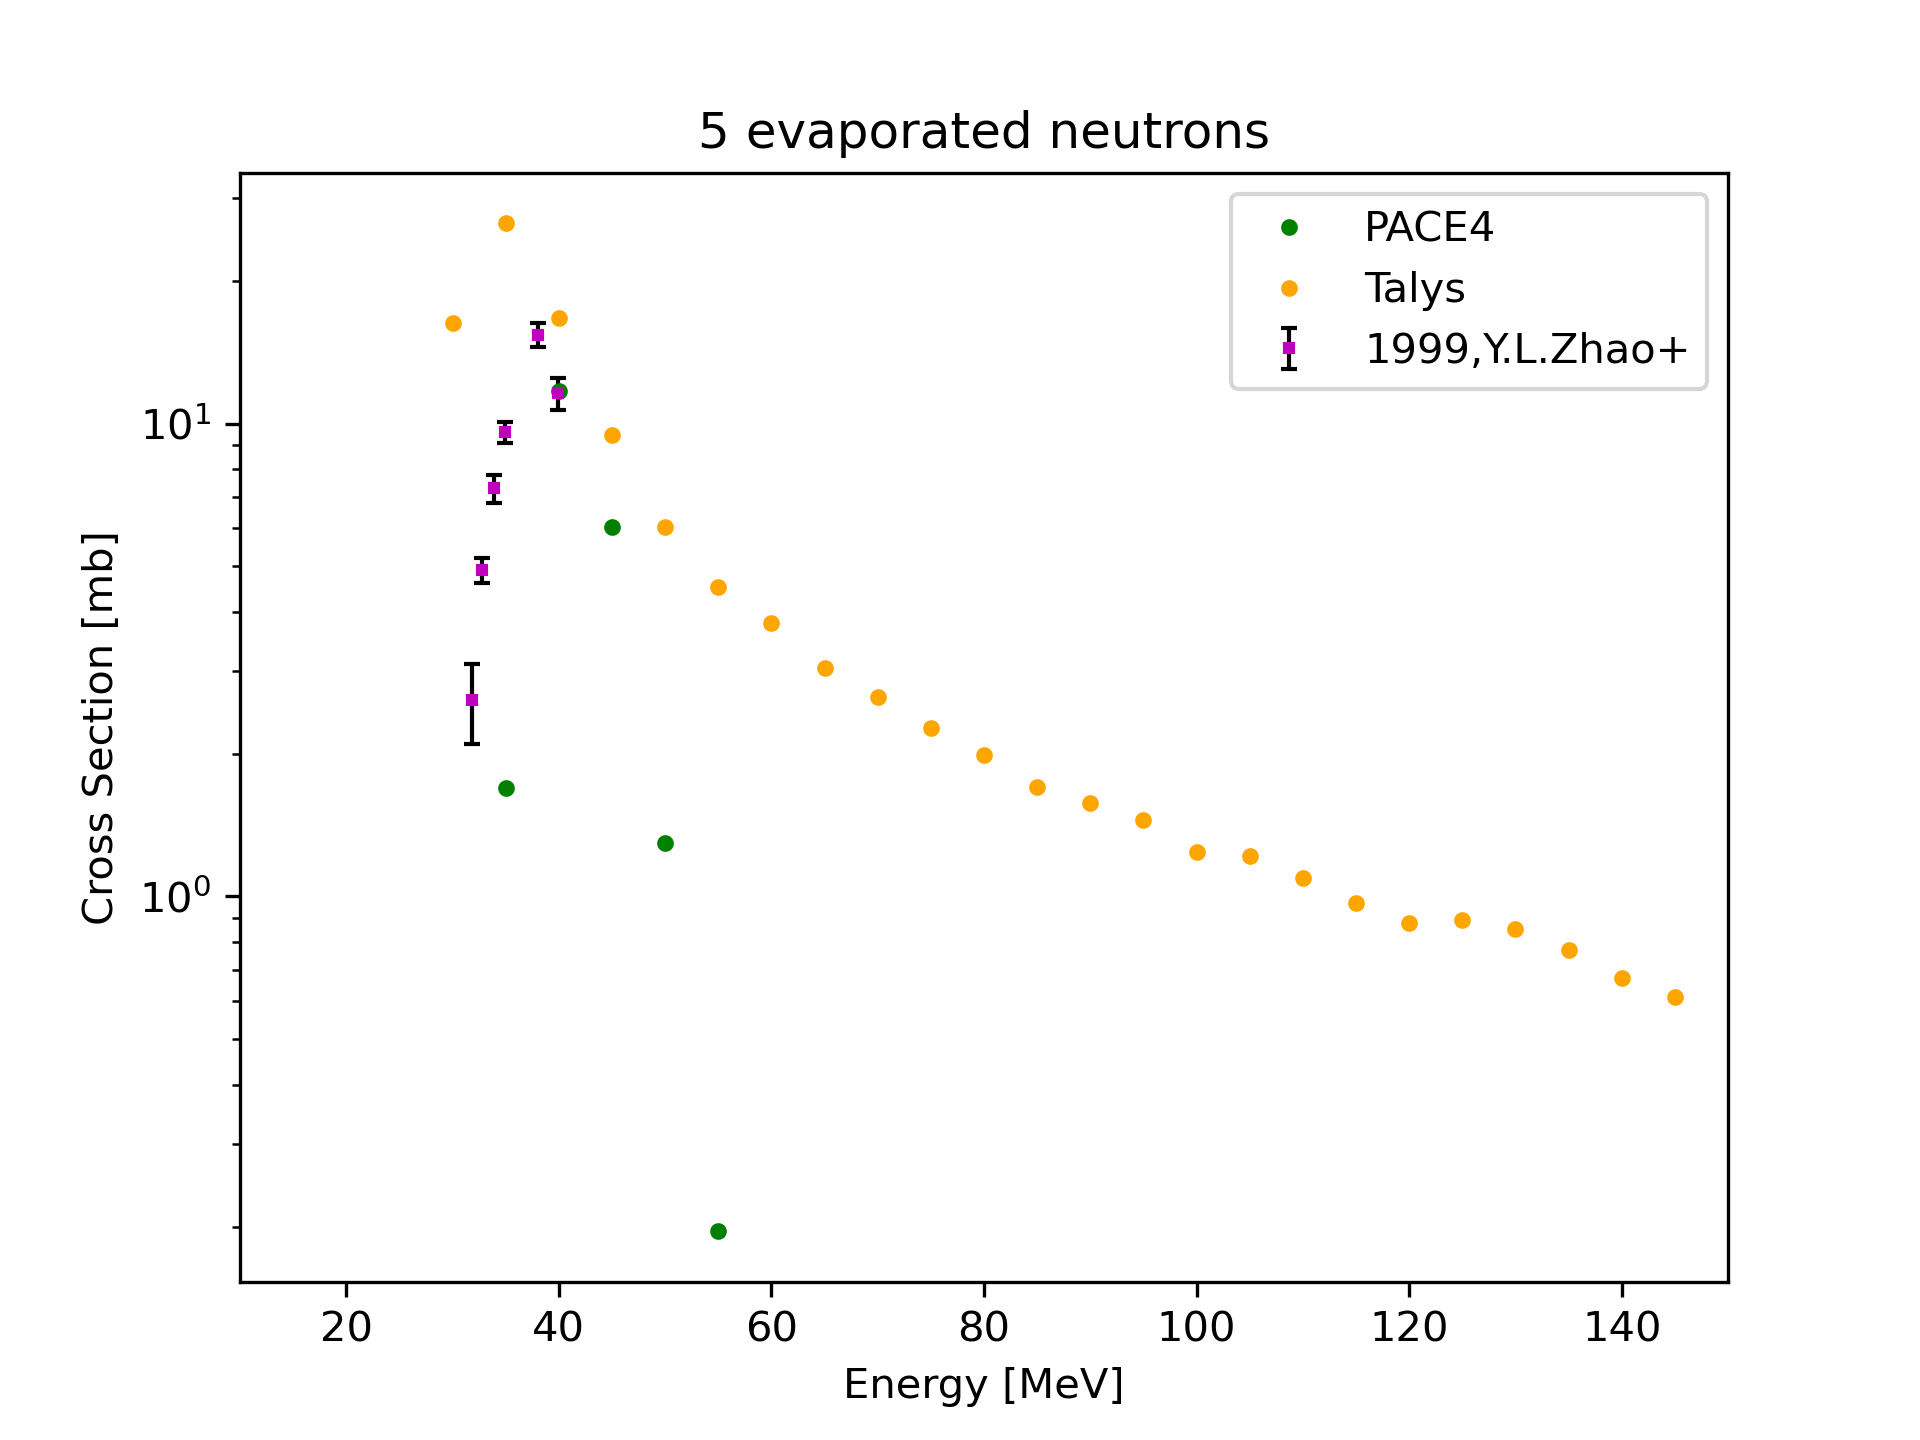
\includegraphics[width=0.9\textwidth]{238U/093234}\\
				\vspace{-0.01\textheight}		
				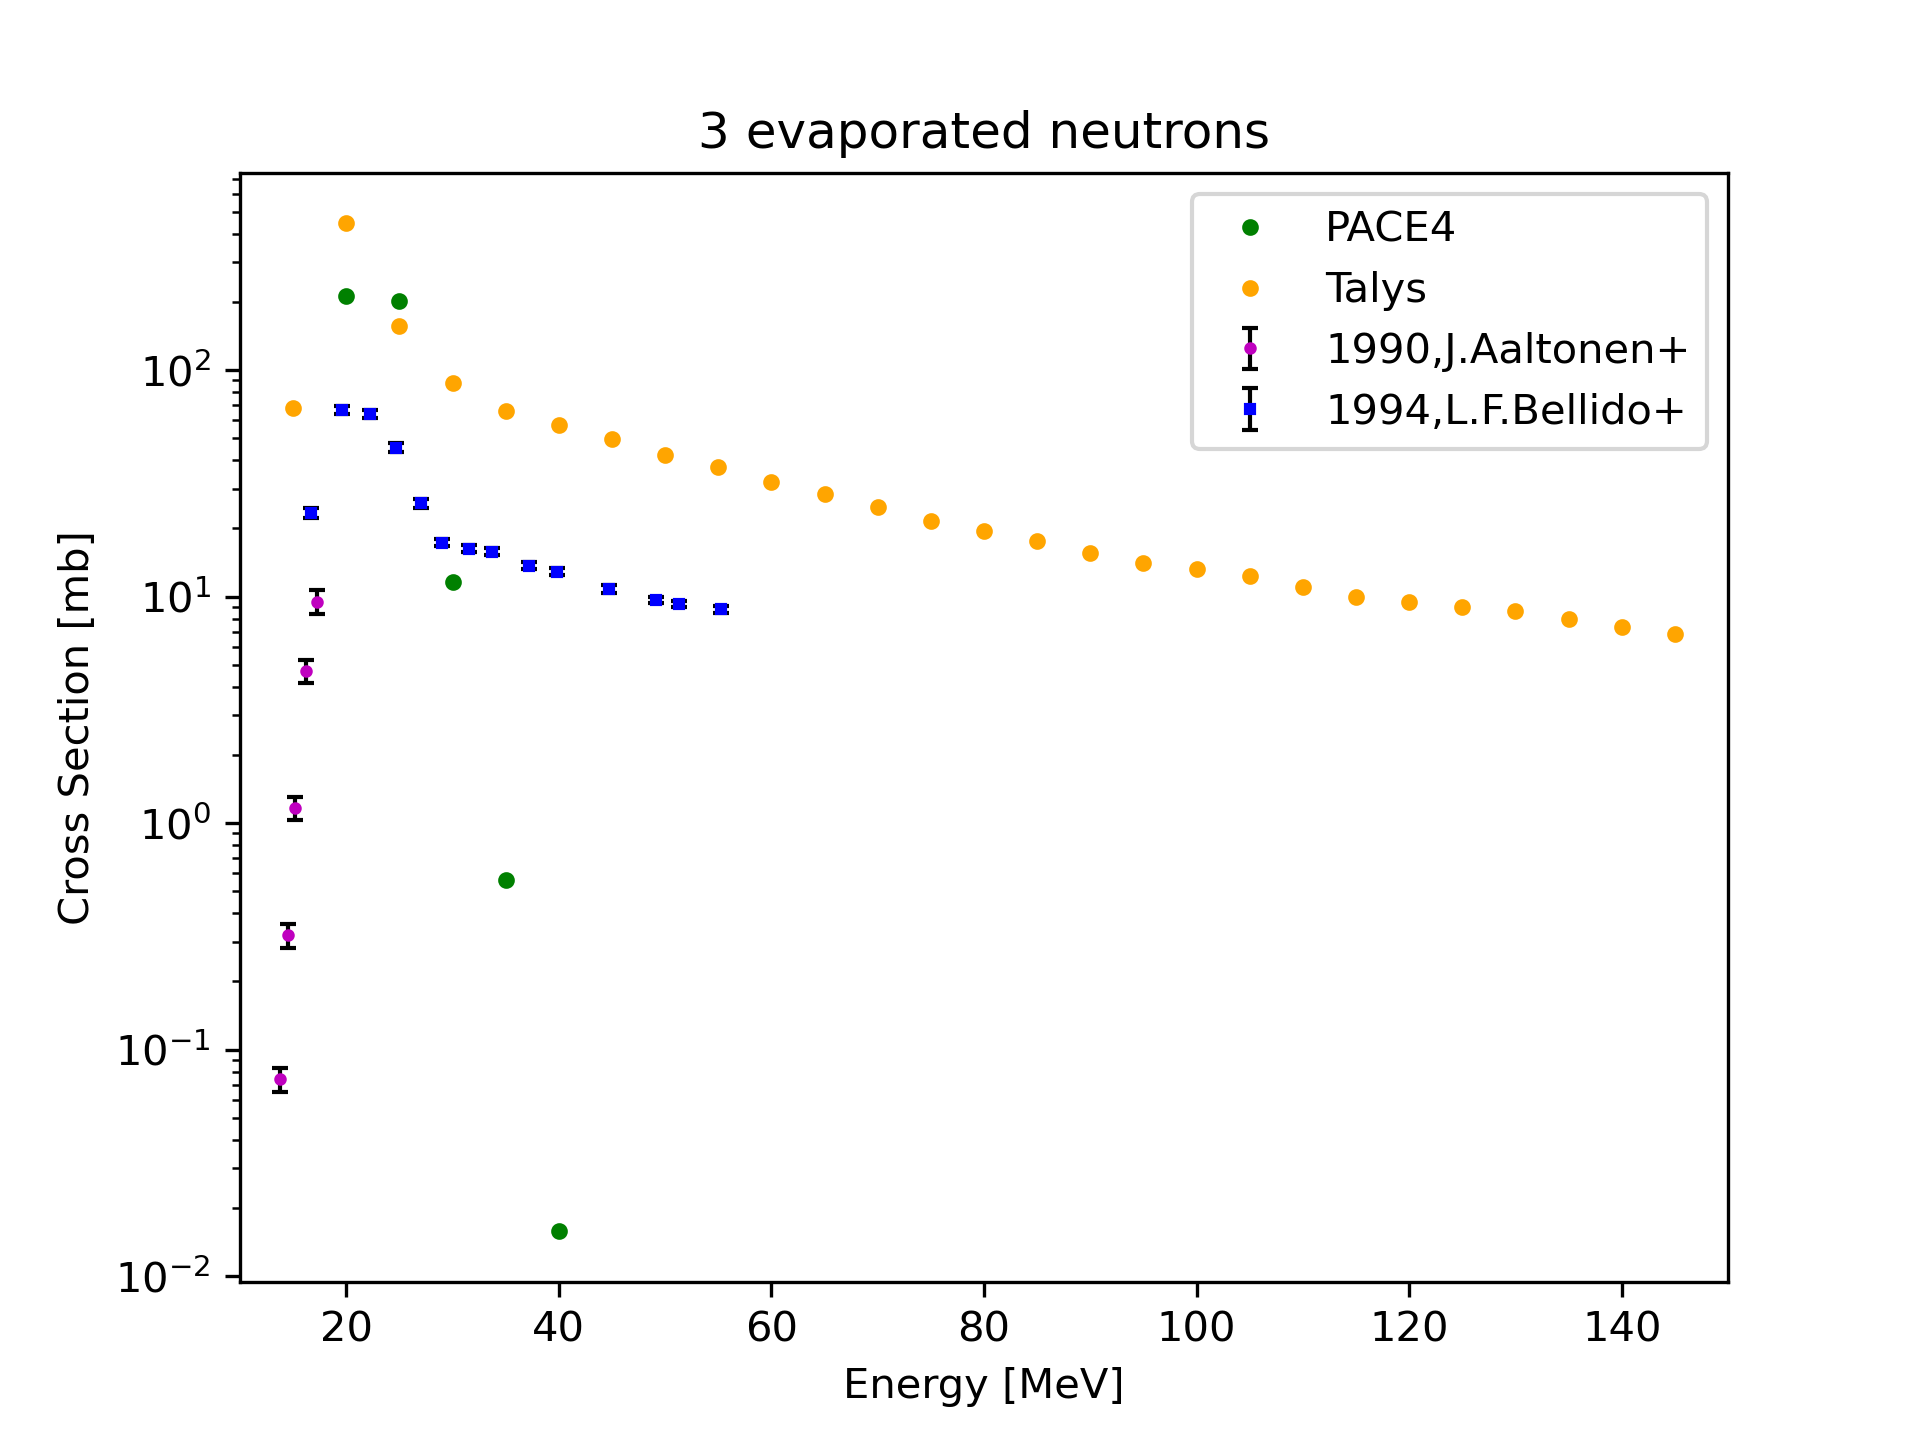
\includegraphics[width=0.9\textwidth]{238U/093236}
			\end{overlayarea}
		\end{column}
		\begin{column}{0.5\textwidth}
			\begin{overlayarea}{\textwidth}{\textheight}
				\centering	    
			   	\vspace{-0.1\textheight}
			   	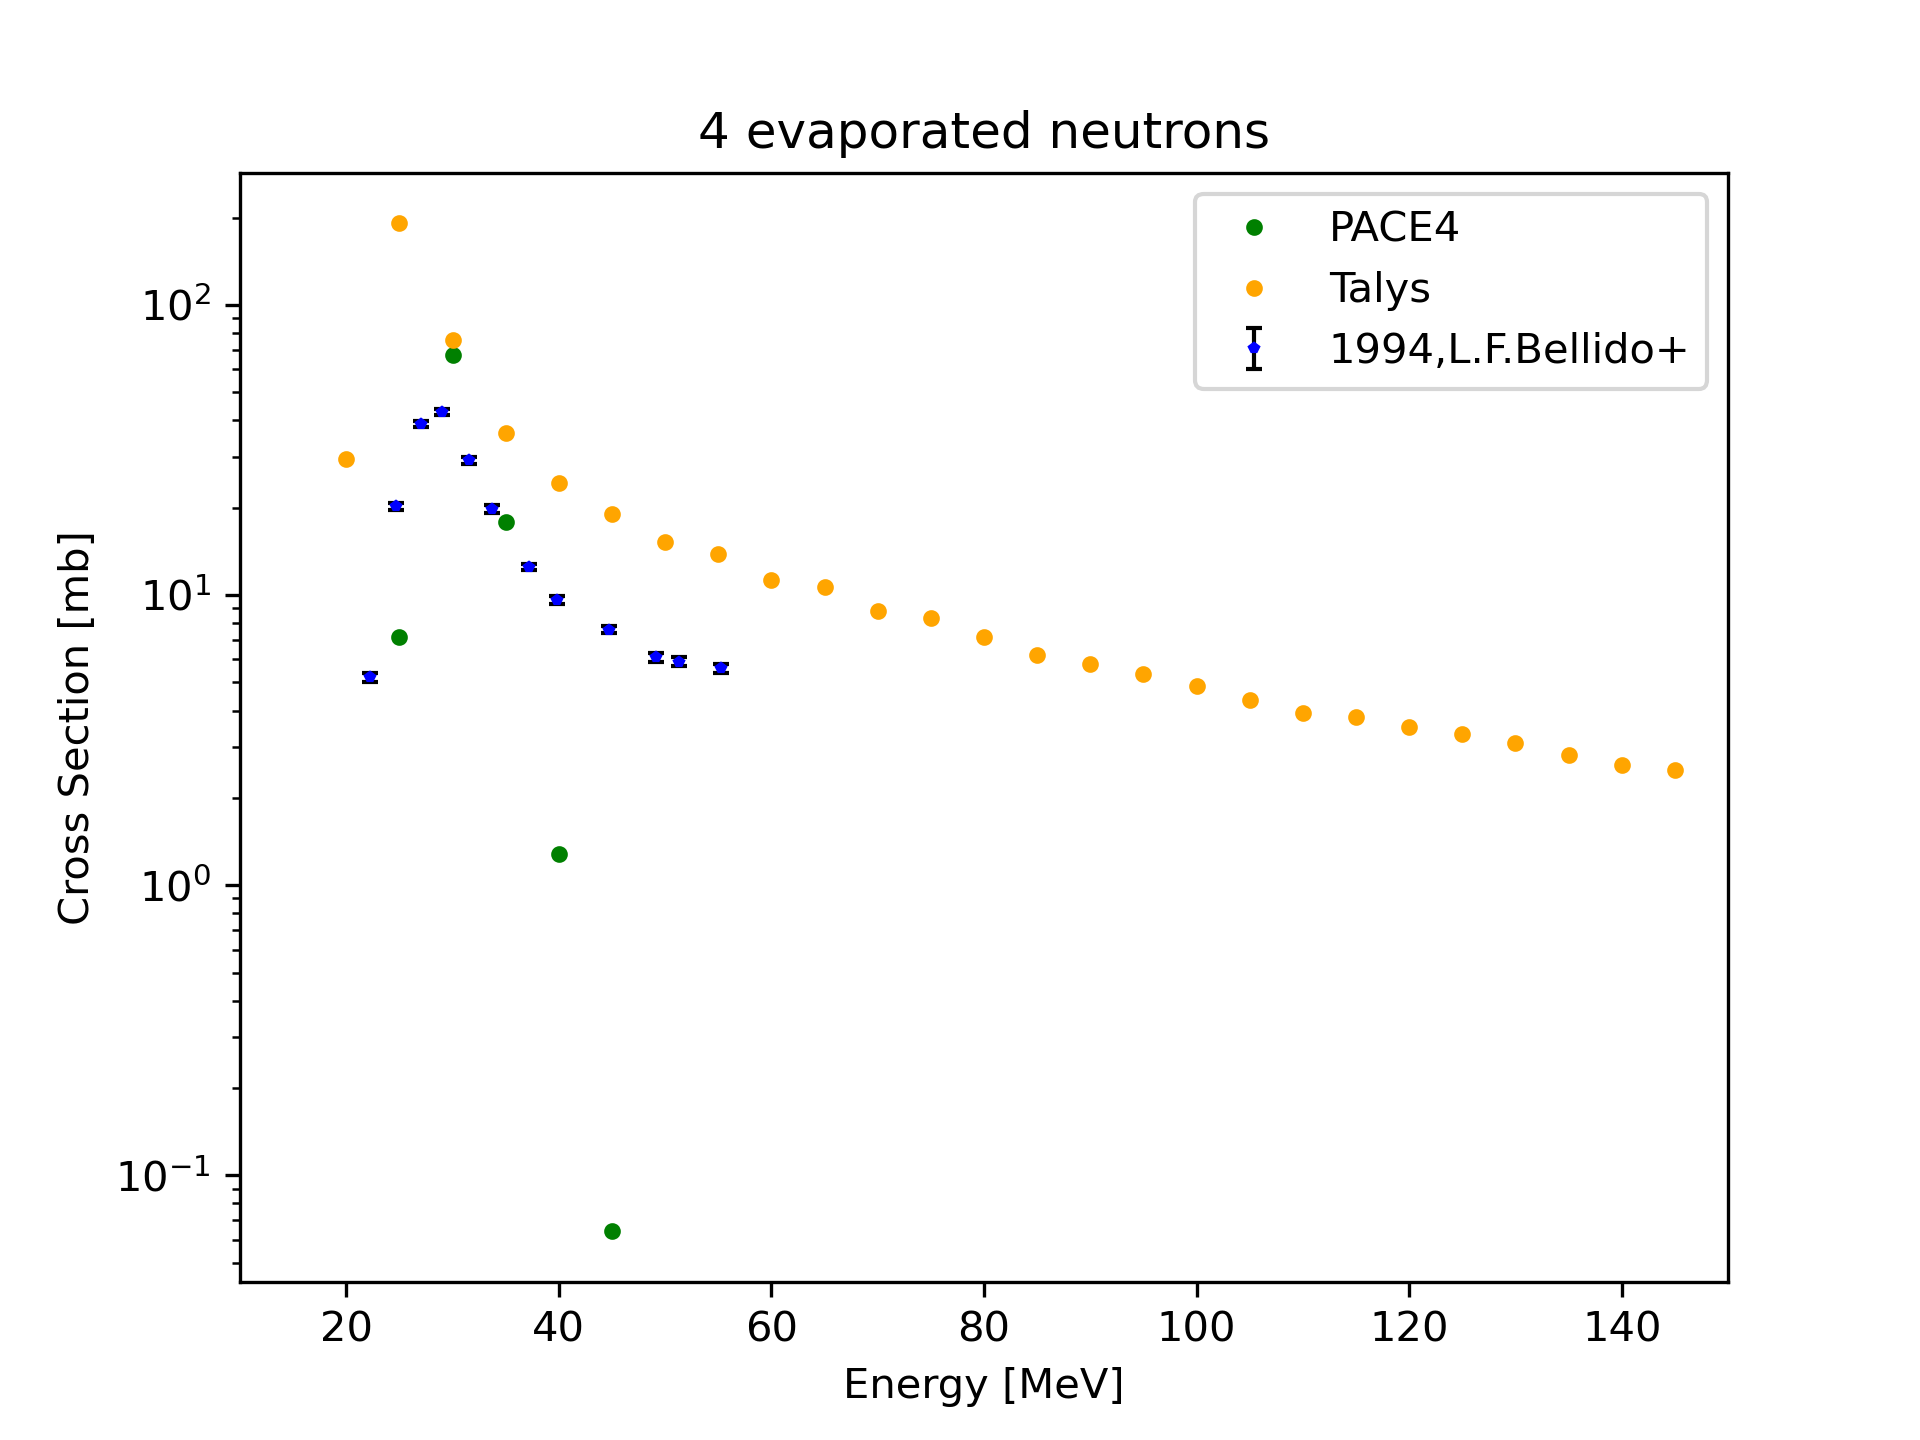
\includegraphics[width=0.9\textwidth]{238U/093235}\\
				\vspace{-0.01\textheight}				
				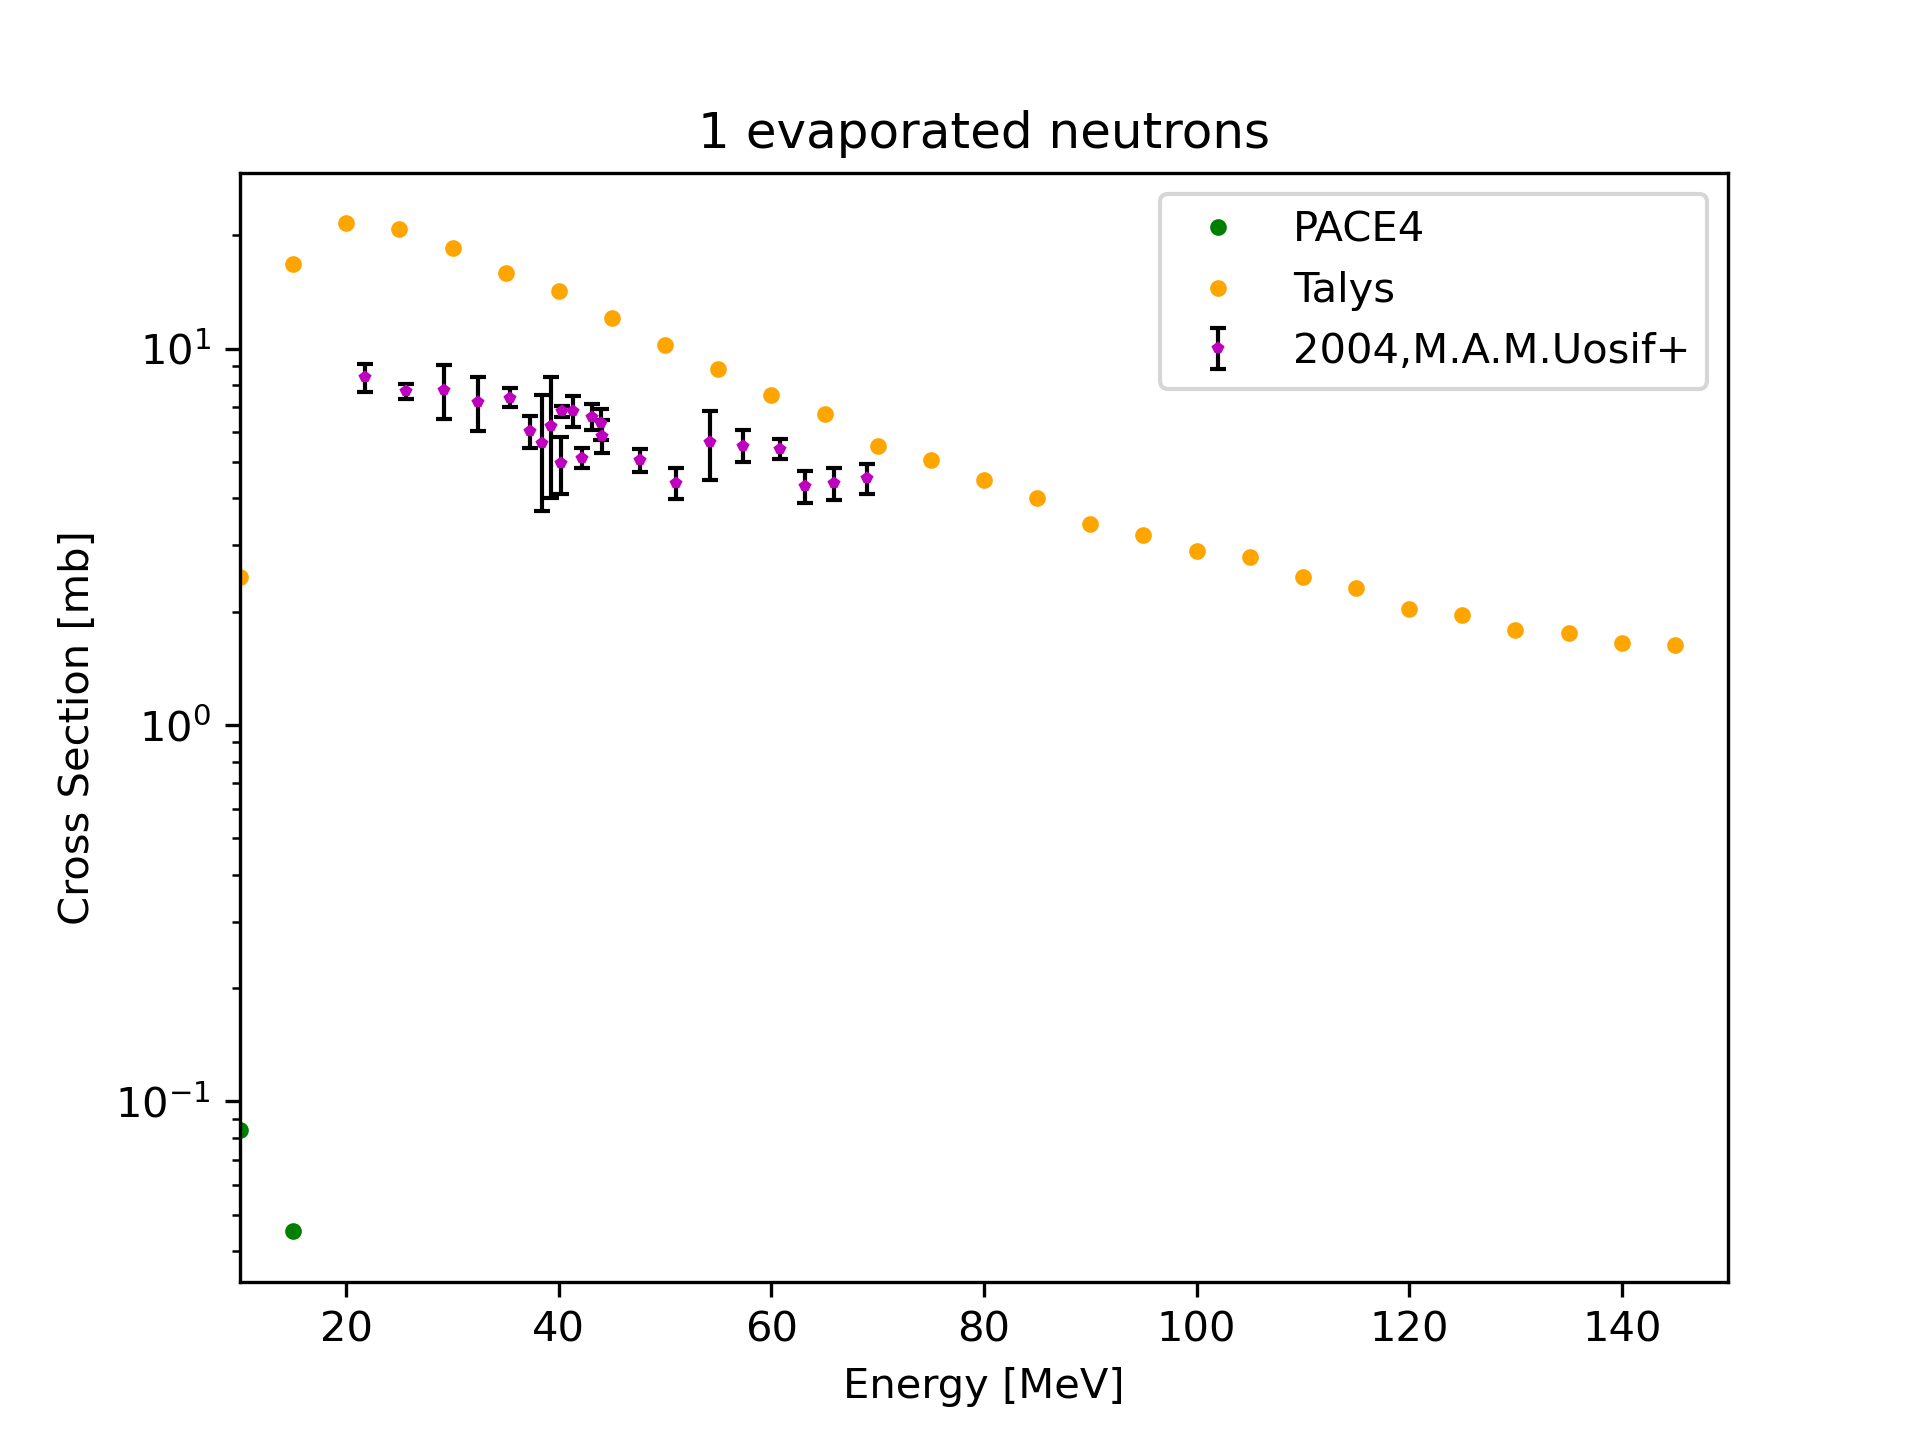
\includegraphics[width=0.9\textwidth]{238U/093238}
			\end{overlayarea}
		\end{column}
	\end{columns}
\end{frame}

\begin{frame}{232Th with 65 MeV protons}
	\begin{columns}
		\begin{column}{0.5\textwidth}
			\begin{overlayarea}{\textwidth}{\textheight}
				\centering	    
			   	\vspace{0.05\textheight}
			   	\textbf{Talys}
			   	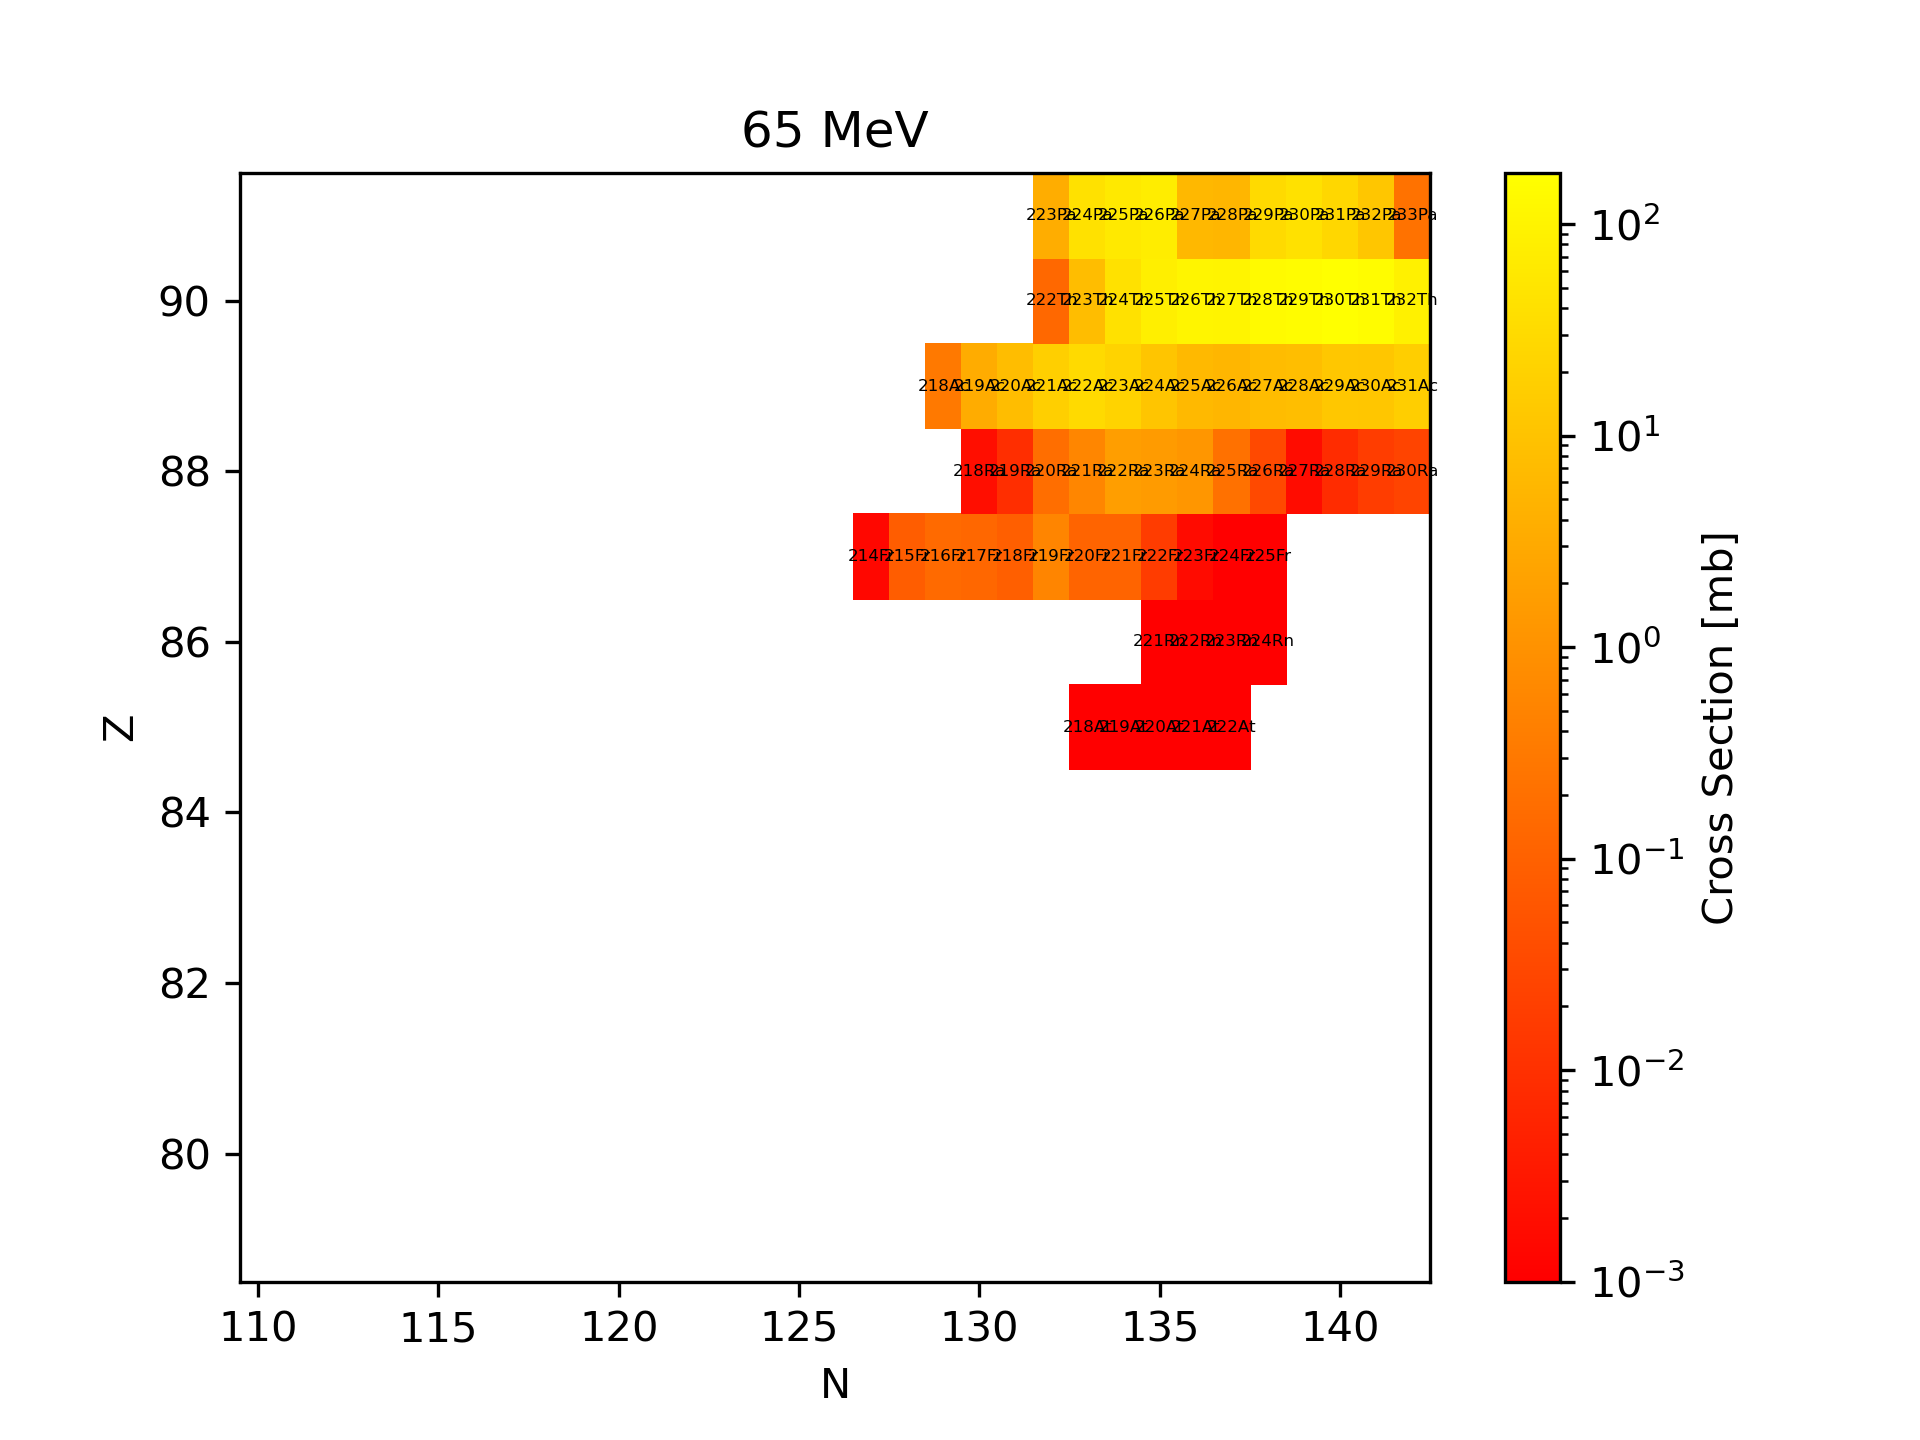
\includegraphics[width=1.1\textwidth]{232Th/Energy_65_Talys}\\
			\end{overlayarea}
		\end{column}
		\begin{column}{0.5\textwidth}
			\begin{overlayarea}{\textwidth}{\textheight}
				\centering	    
			   	\vspace{0.05\textheight}
			   	\textbf{PACE4}
				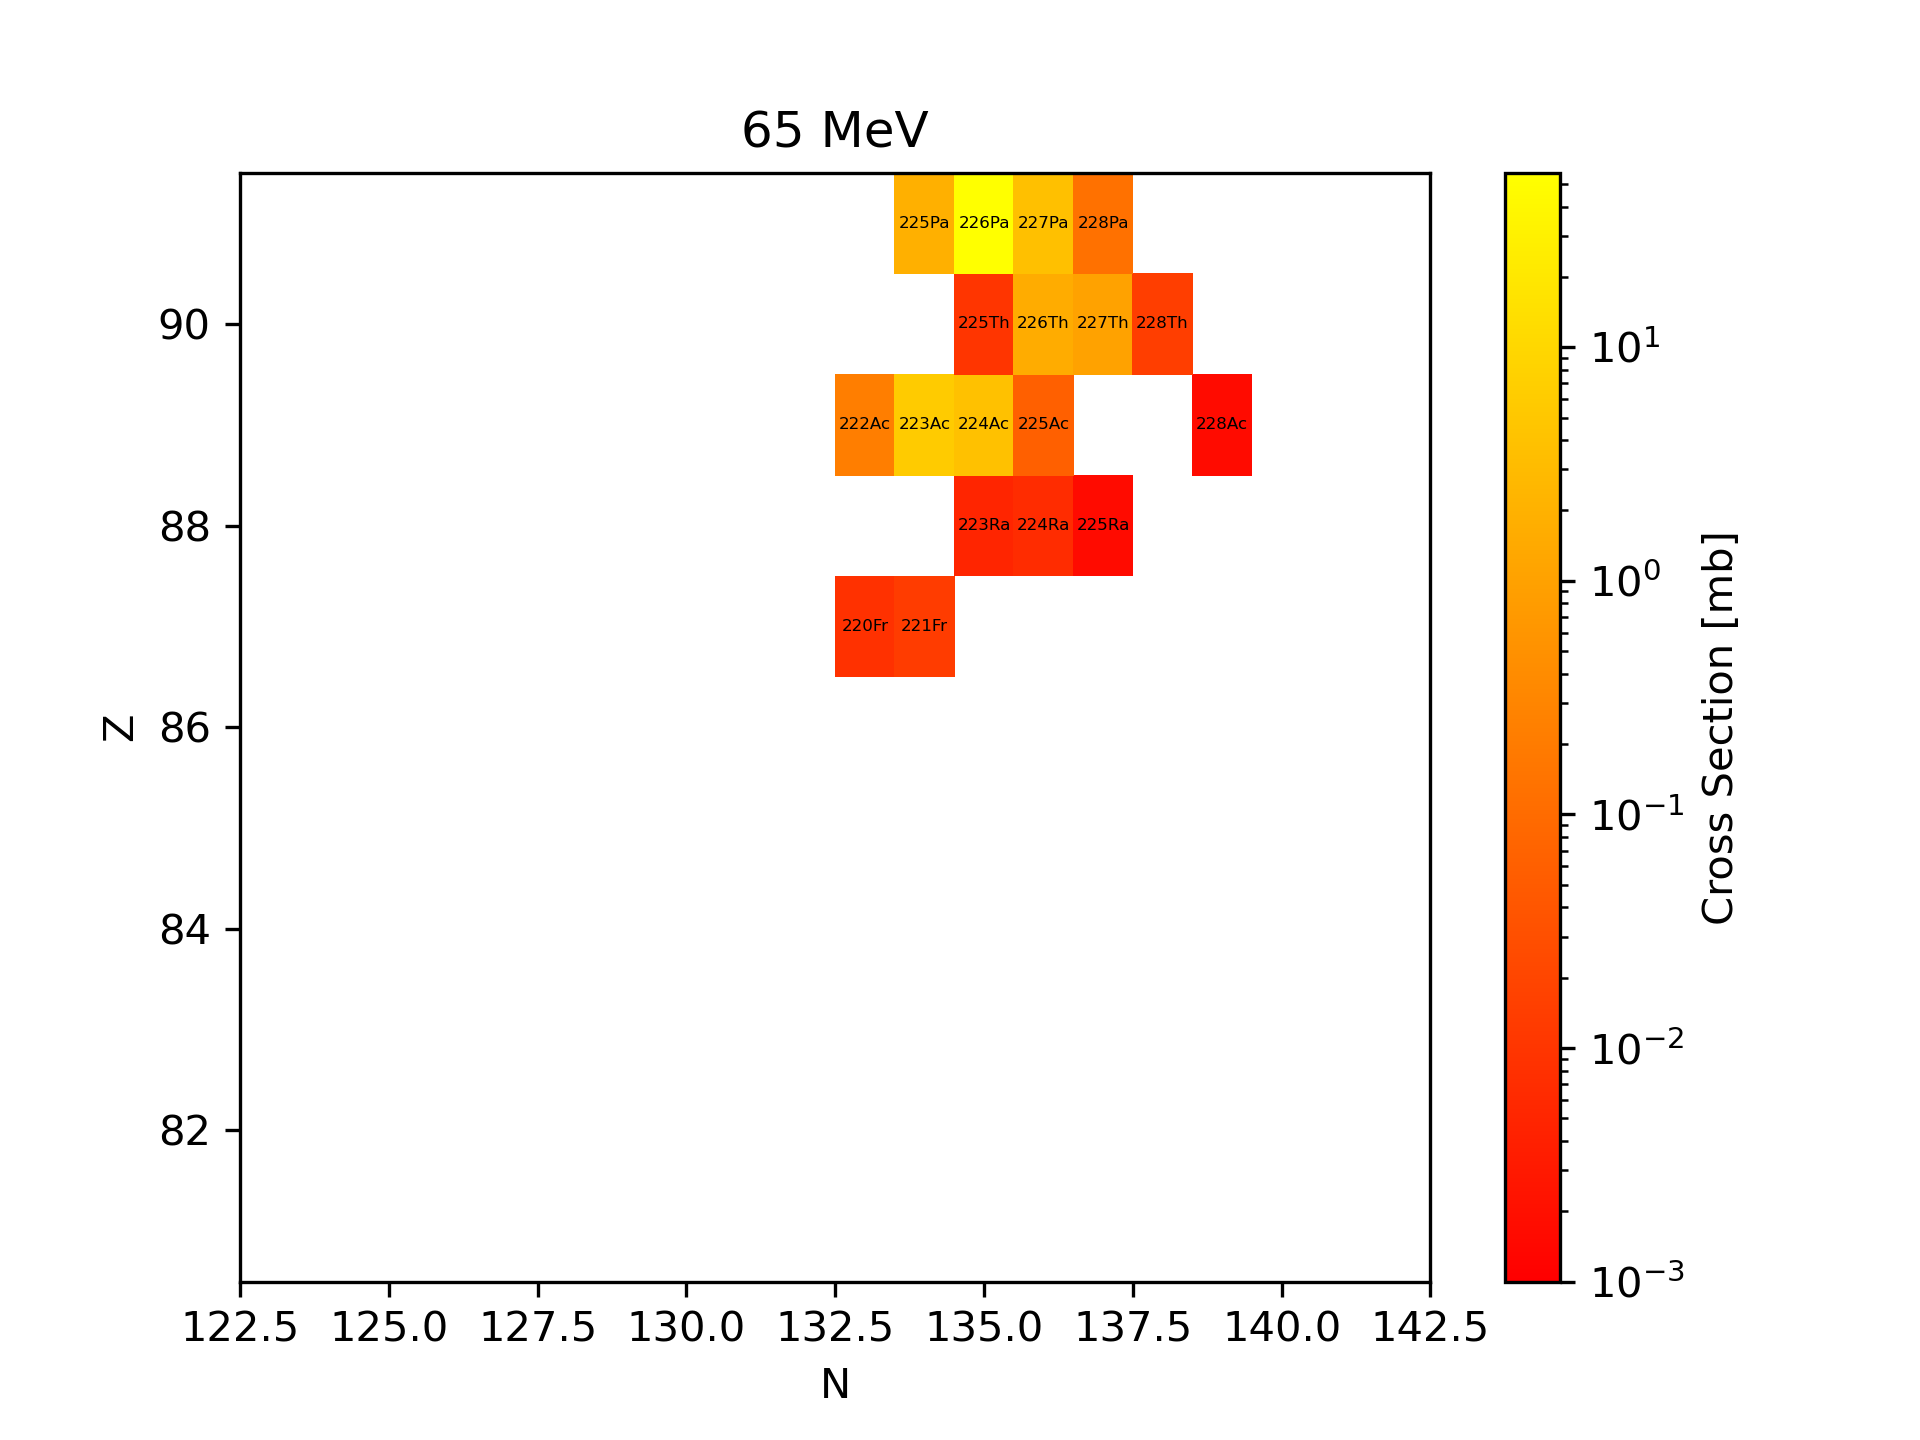
\includegraphics[width=1.1\textwidth]{232Th/Energy_65_Pace}
			\end{overlayarea}
		\end{column}
	\end{columns}
\end{frame}


\begin{frame}{233U with 65 MeV protons}
	\begin{columns}
		\begin{column}{0.5\textwidth}
			\begin{overlayarea}{\textwidth}{\textheight}
				\centering	    
			   	\vspace{0.05\textheight}
			   	\textbf{Talys}
			   	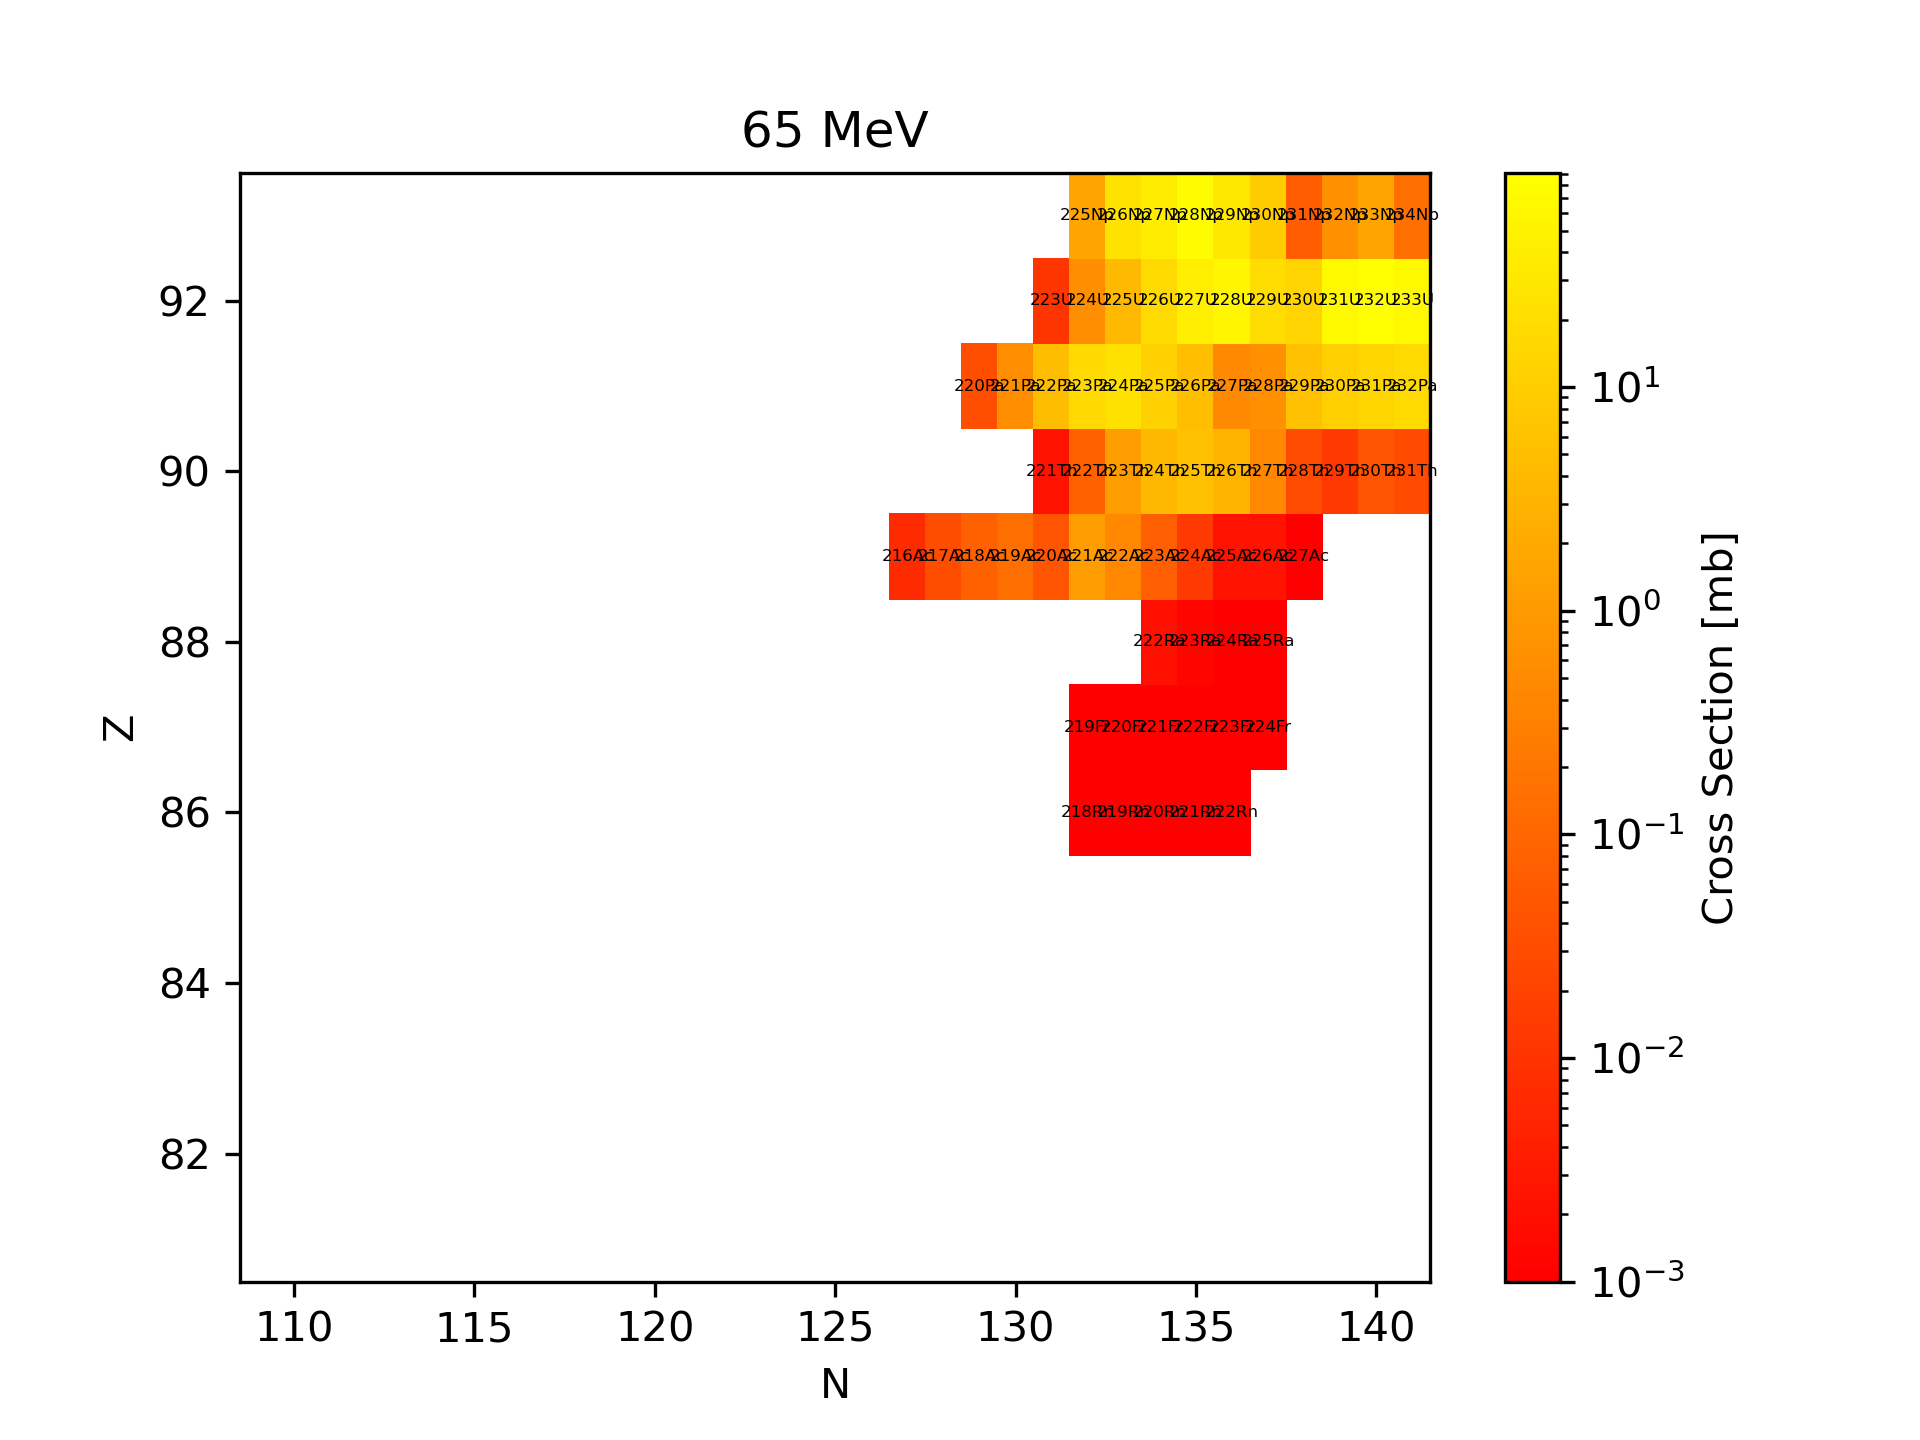
\includegraphics[width=1.1\textwidth]{233U/Energy_65_Talys}\\
			\end{overlayarea}
		\end{column}
		\begin{column}{0.5\textwidth}
			\begin{overlayarea}{\textwidth}{\textheight}
				\centering	    
			   	\vspace{0.05\textheight}
			   	\textbf{PACE4}
				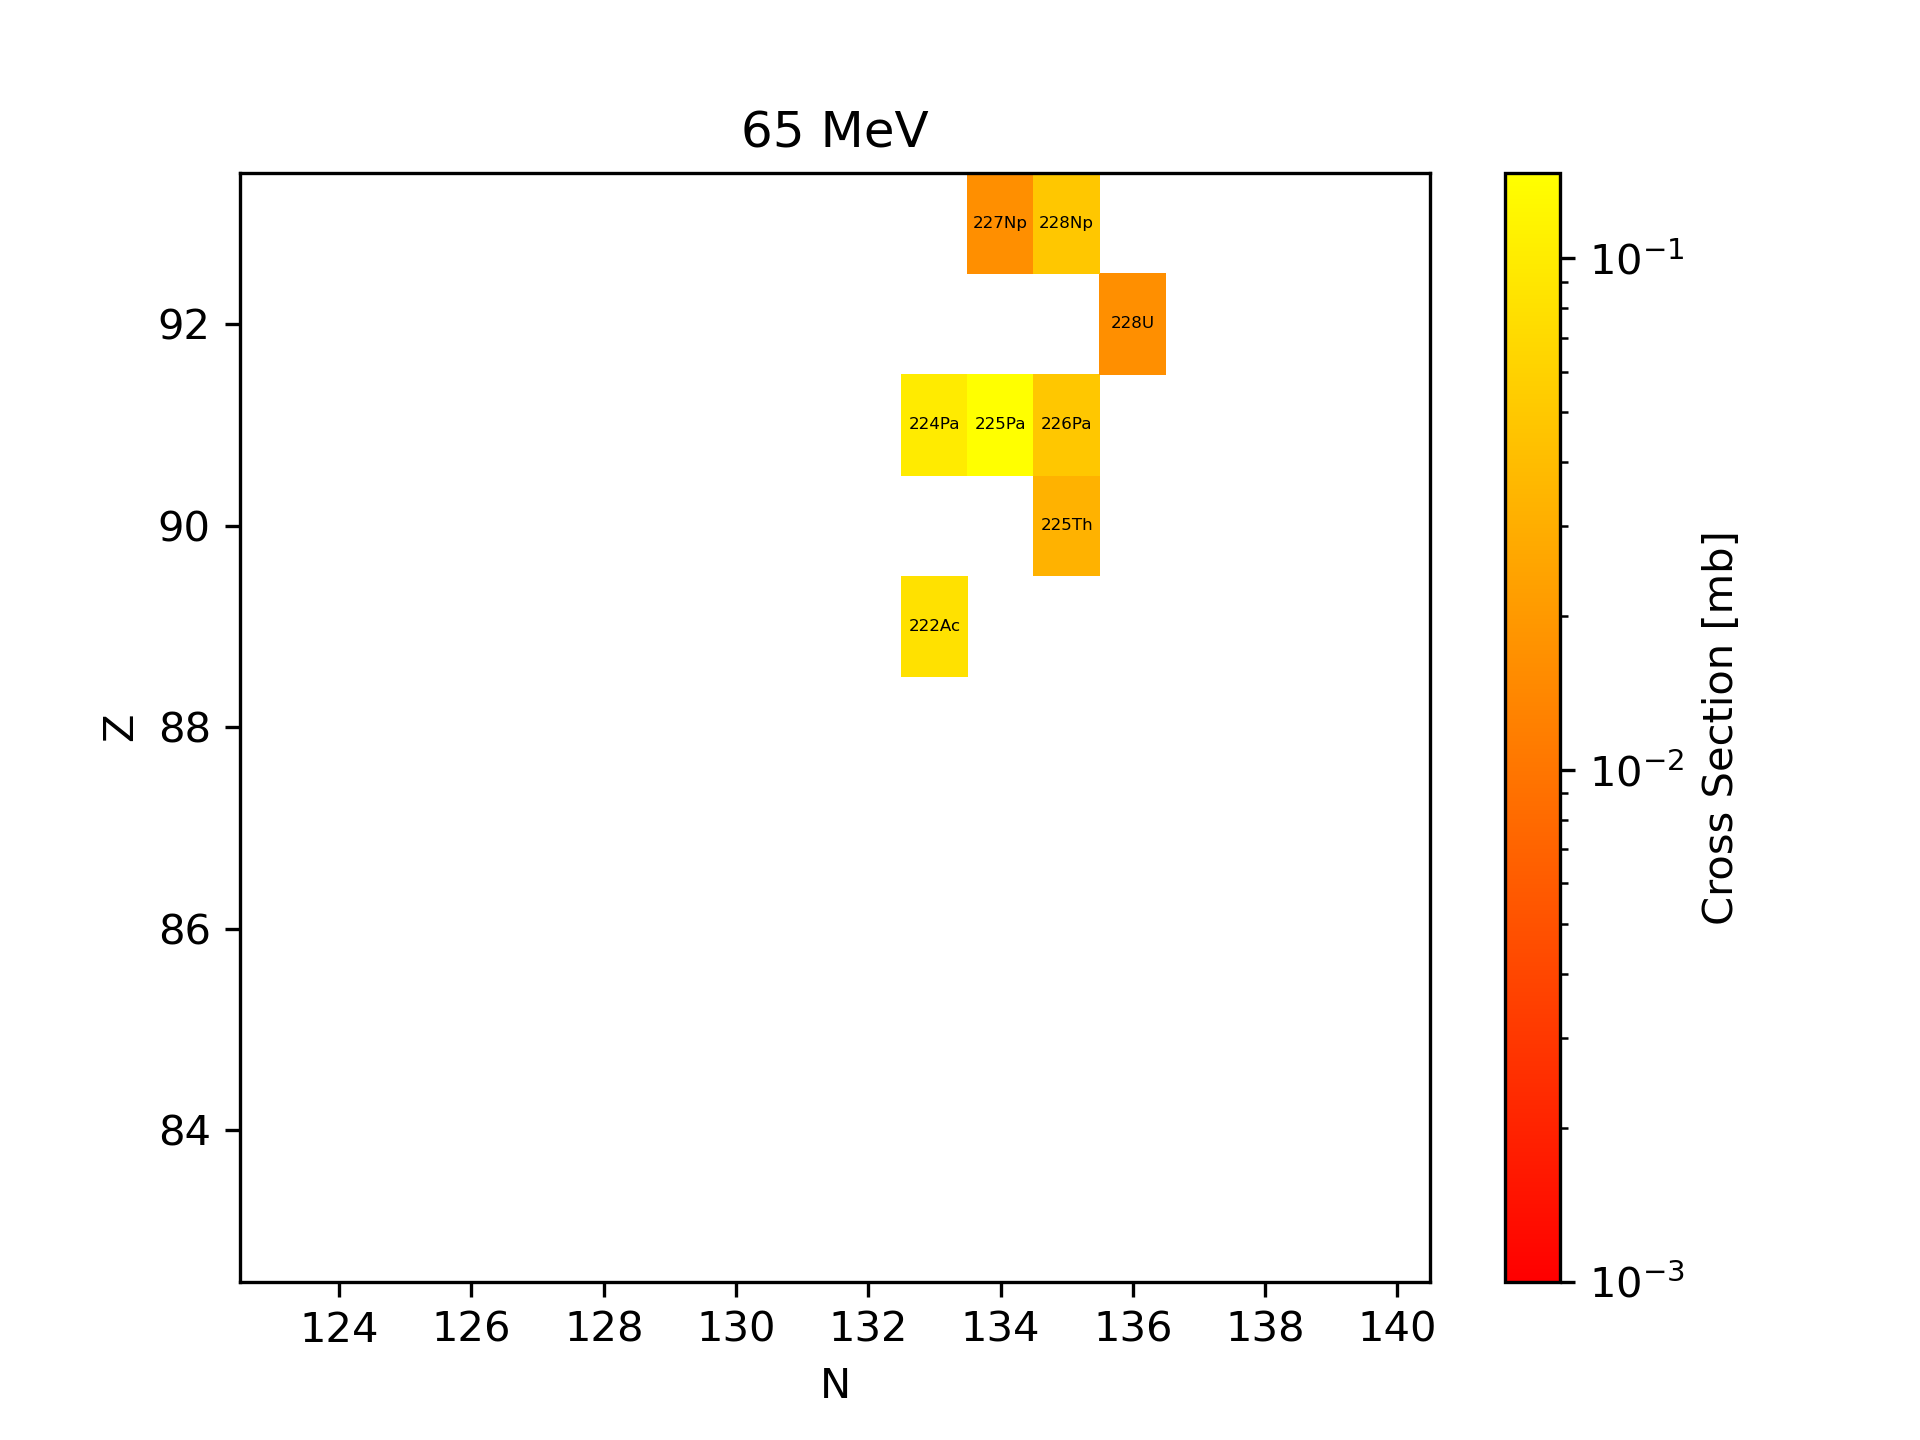
\includegraphics[width=1.1\textwidth]{233U/Energy_65_Pace}
			\end{overlayarea}
		\end{column}
	\end{columns}
\end{frame}

\begin{frame}{238U with 65 MeV protons}
	\begin{columns}
		\begin{column}{0.5\textwidth}
			\begin{overlayarea}{\textwidth}{\textheight}
				\centering	    
			   	\vspace{0.05\textheight}
			   	\textbf{Talys}
			   	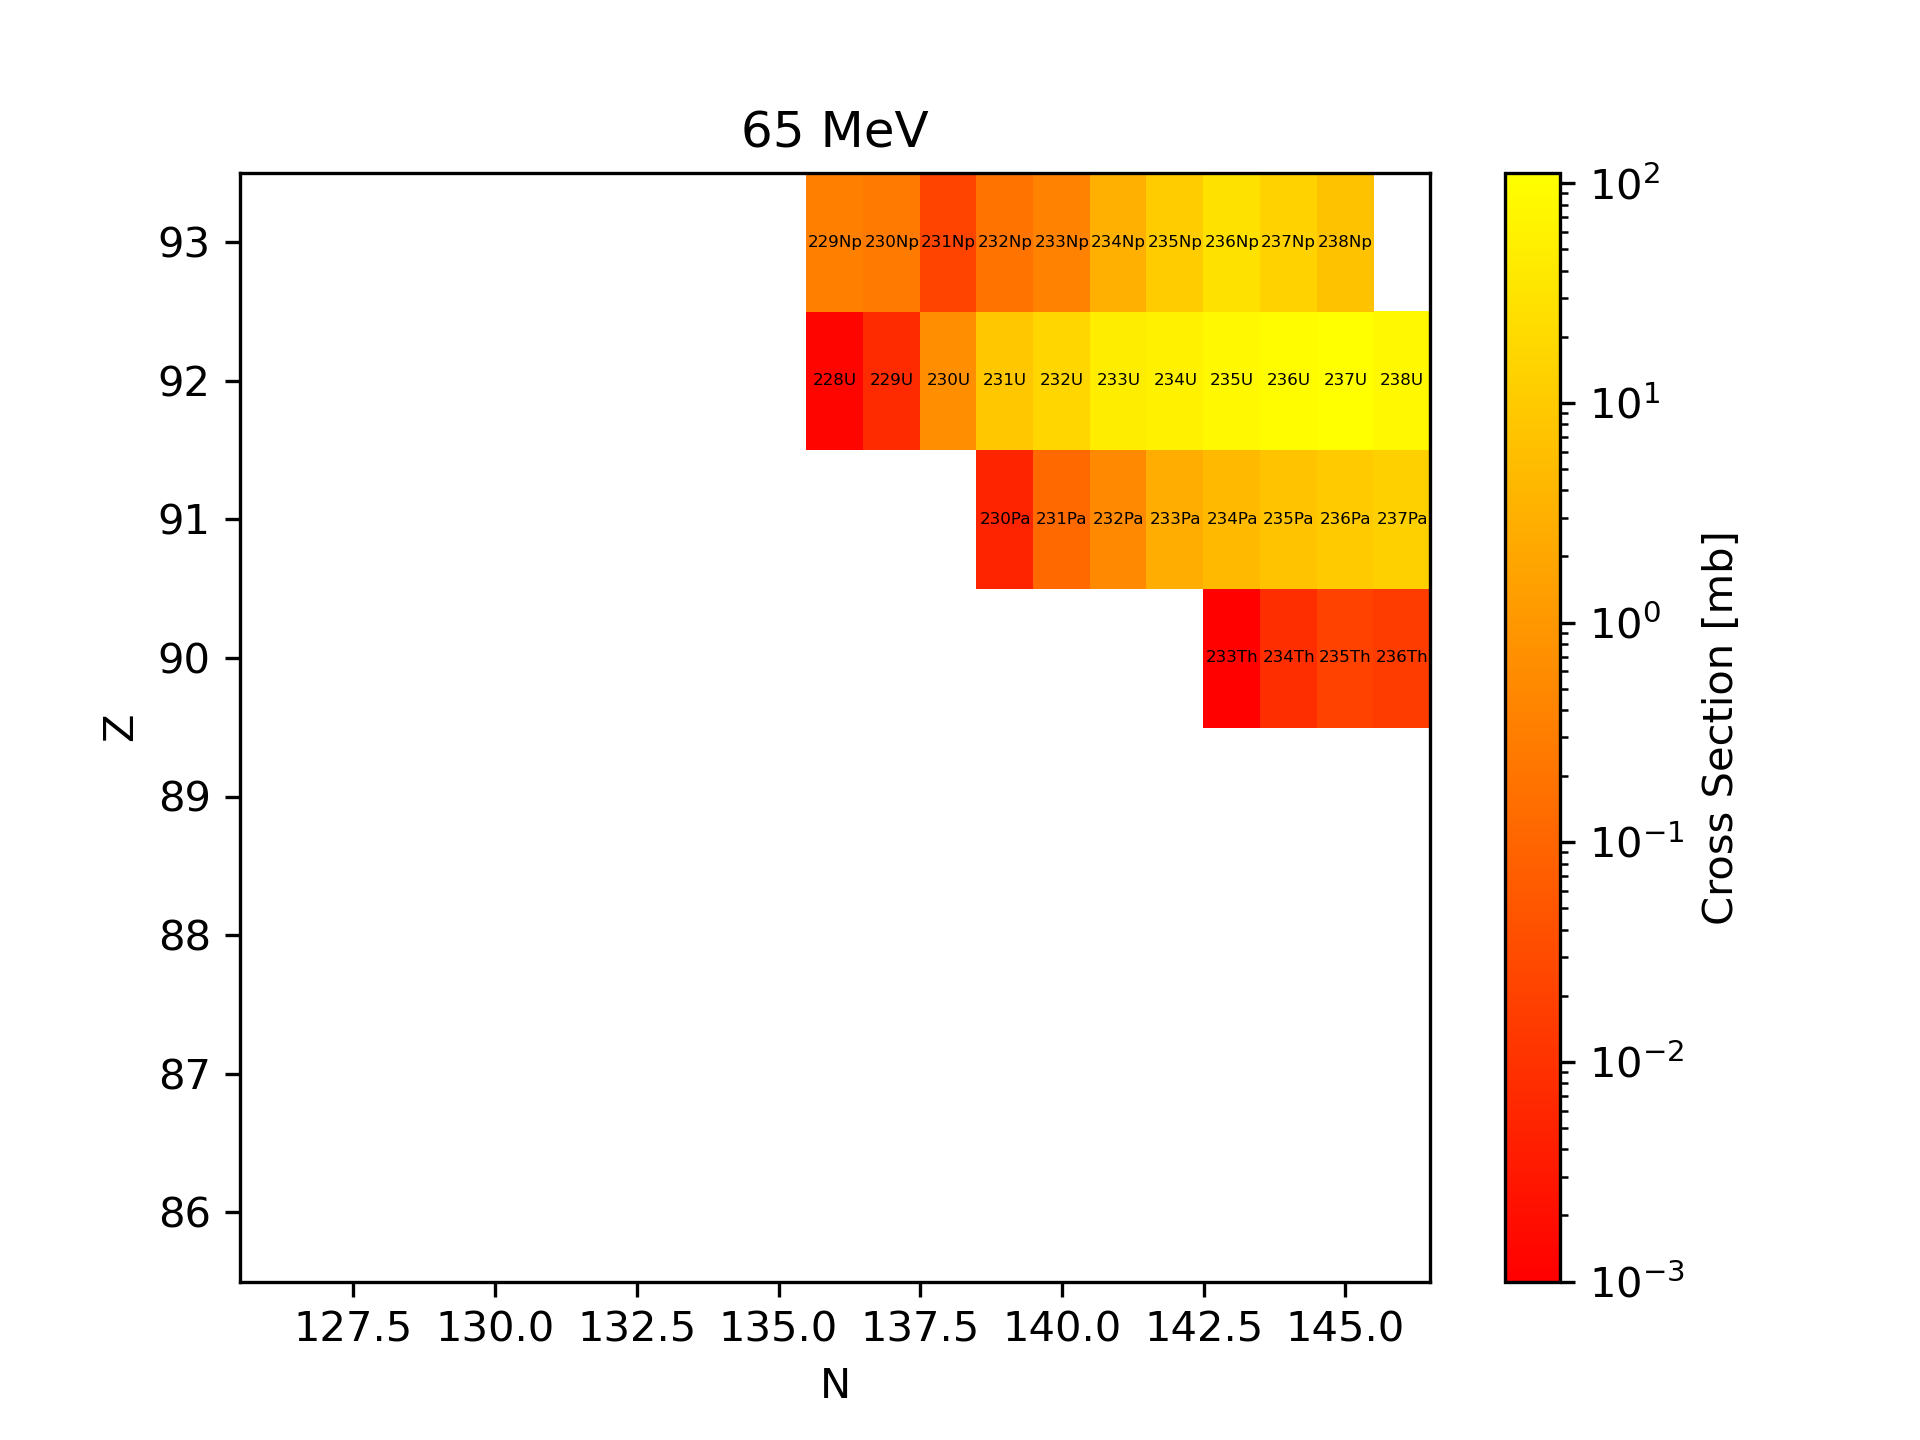
\includegraphics[width=1.1\textwidth]{238U/Energy_65_Talys}\\
			\end{overlayarea}
		\end{column}
		\begin{column}{0.5\textwidth}
			\begin{overlayarea}{\textwidth}{\textheight}
				\centering	    
			   	\vspace{0.05\textheight}
			   	\textbf{PACE4}
				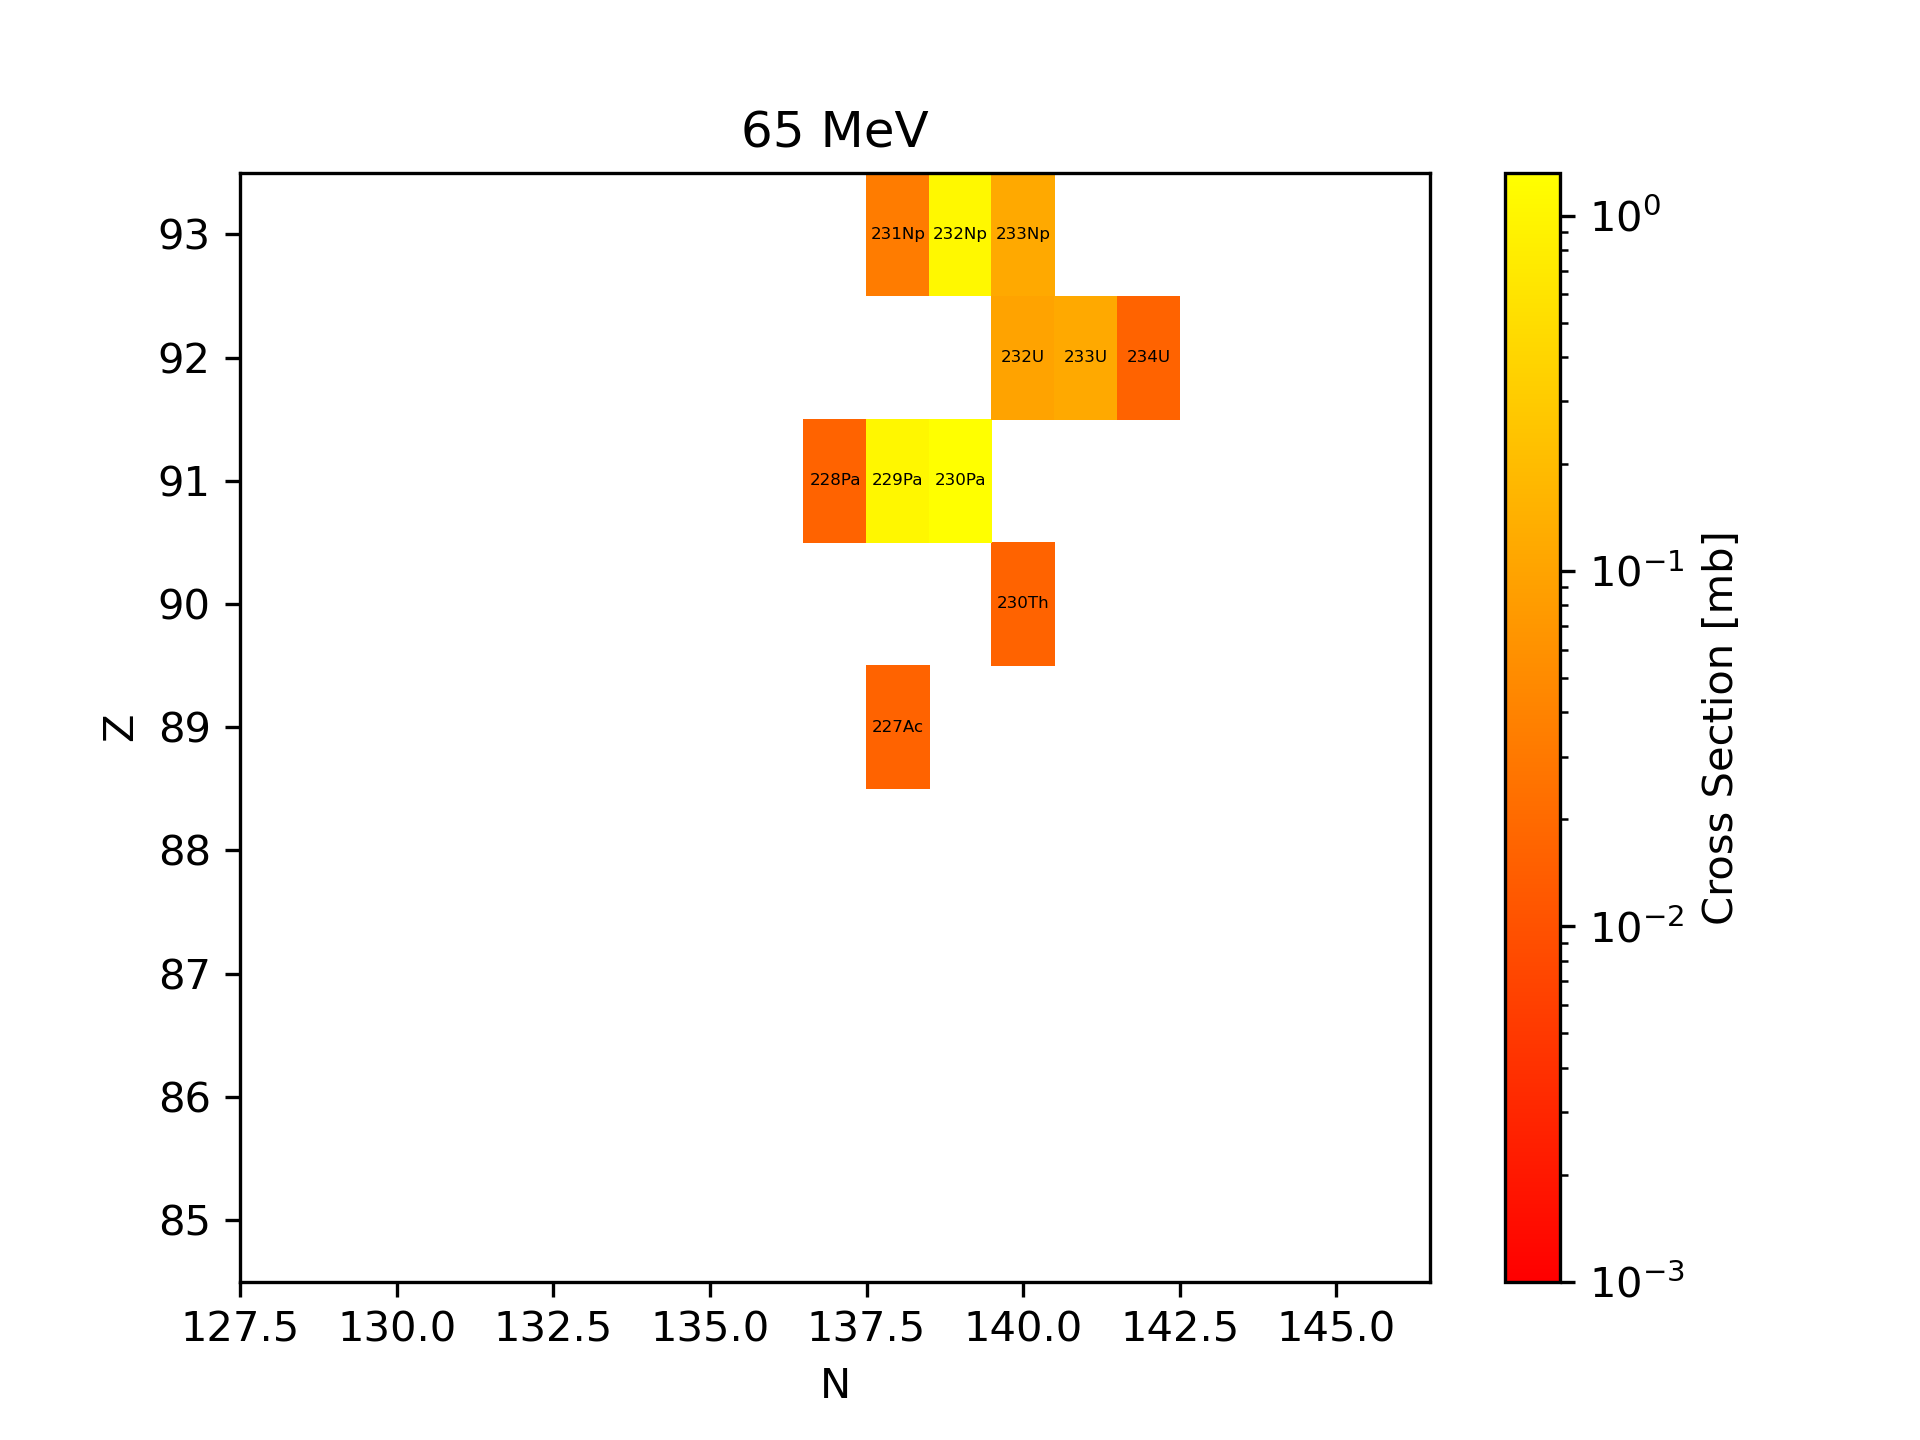
\includegraphics[width=1.1\textwidth]{238U/Energy_65_Pace}
			\end{overlayarea}
		\end{column}
	\end{columns}
\end{frame}



\end{document}